\documentclass[a4paper, 10pt, fleqn]{article}
\setlength{\mathindent}{0pt}
\usepackage{amsmath}
\usepackage{amssymb}
\usepackage[justification=centering]{caption}
\usepackage[margin=0.75in]{geometry}
\usepackage{graphicx}
\usepackage{float}
\usepackage{multirow}
\usepackage[table]{xcolor}
\usepackage{hyperref}
\usepackage{subcaption}
\usepackage{tabularx}
\usepackage{titlesec}


\titleformat{\section}[block]{\normalfont\Large\bfseries\centering}{\thesection}{1em}{}

\begin{document}

   \begin{titlepage}
      \centering

      \vspace*{2cm}
      
\includegraphics[width=0.48\linewidth]{../img/UCT logo circular blue large.png}

      \vspace*{2cm}

      {\LARGE GAUSSIAN PROCESSES FOR TIME SERIES \\[0.5em]
      with application to air pollution forecasting}

      \vspace*{2cm}

      {\large Raphaela Azar \& Sbonelo Gumede}

      \vspace*{2cm}
      
      \begin{large}
         Minor dissertation presented in partial fullfilment of the requirements for the degree of Honours in Statistics \& Data Science
      \end{large}

      \vspace*{2cm}

      \begin{large}
         Department of Statistical Sciences\\
         University of Cape Town
      \end{large}

      \vspace*{2cm}

      Supervised by\\
      Dr Birgit Erni

      \vfill

   \end{titlepage}

   \begin{flushleft}

   \section*{Abstract}

    In this paper we give a basic introduction into Gaussian Processes. We delve into how can you use a Gaussian process for time series analysis. Compare the peformance of Gaussian processes to other time series models. An area of application included is predicting the level of air pollution in the Table View station in Cape Town for the year of 2019. Another area of application is predicting the gold price for South Africa for the year of 2020. This is done in a Bayesian framework in order to make probabilistic statements and obtain a predictive distribution for future forecasts.

   \section*{Literature Review}

   ((\hyperref[Rasmussen2006]{Rasmussen and Williams, 2006})) We have a training set of $\mathcal{D}$ of $n$ observations, $\mathcal{D} = \{(\mathbf{x}_{i}, y_{i}) \, | \, i = 1, \, \ldots, \, n\}$, where $\mathbf{x}$ denotes the input vector (covariates) of dimension $\mathcal{D}$ and y denotes a scalar output or target (dependent variable); the column vector of inputs for all n cases are arranged in the $\mathcal{D} \times n \, design \, matrix\, X$, and the targets are collected in the vector $\mathbf{y}$, so we can write $\mathcal{D} = (X, \mathbf{y})$. 

   \vspace{1em}

   \textbf{Definition 2.1.1} ((\hyperref[Rasmussen2006]{Rasmussen and Williams, 2006})).
   \textit{A Gaussian process is a collection of random variables, any finite number of which have a joint Gaussian distribution.}

   \vspace{1em}

   A Gaussian process is completely specified by its mean function and co-variance function. We define mean mean function $m(\mathbf{x})$ and the covariance function $k(\mathbf{x}, \mathbf{x}')$ for a real process $f(\mathbf{x})$ as
   $$m(\mathbf{x}) = \mathbb{E}[f(\mathbf{x})],$$
   $$k(\mathbf{x}, \mathbf{x}') = \mathbb{E}[(f(\mathbf{x}) - m(\mathbf{x}))(f(\mathbf{x}') - m(\mathbf{x}'))],$$
   and will write the Gaussian process as
   $$f(\mathbf{x}) \sim \text{GP}(m(\mathbf{x}), \, k(\mathbf{x}, \mathbf{x}')).$$

   $\mathbf{x} =
   \begin{bmatrix}
      X_{1} \\
      \vdots \\
      X_{p}
   \end{bmatrix}
   \:
   \sim \mathcal{N}_{p}(\mathbf{m}, \, \mathbf{K}),
   \:
   \text{where}
   \:
   \mathbf{m} = 
   \begin{bmatrix}
      m(x_{1}) \\
      m(x_{2}) \\
      \vdots \\
      m(x_{p})
   \end{bmatrix}  
   \: 
   \text{and}
   \:
   \mathbf{K} = 
   \begin{bmatrix}
      k(x_{1}, \, x_{1}) & k(x_{1}, \, x_{2}) & \cdots & k(x_{1}, \, x_{p}) \\
      k(x_{2}, \, x_{1}) & k(x_{2}, \, x_{2}) & \cdots & k(x_{2}, \, x_{p}) \\
      \vdots & \vdots & \ddots & \vdots \\
      k(x_{p}, \, x_{1}) & k(x_{p}, \, x_{2}) & \cdots & k(x_{p}, \, x_{p})
   \end{bmatrix}$.
   
   \vspace{1em}

   Consider a simple example shown in Figure~\ref{figure_1}, where $m(\mathbf{x}) = \mathbf{x} \, \text{and} \, k(\mathbf{x}, \mathbf{x}') = \text{I}_{p}$. 

   \begin{figure}[H]
      \centering
      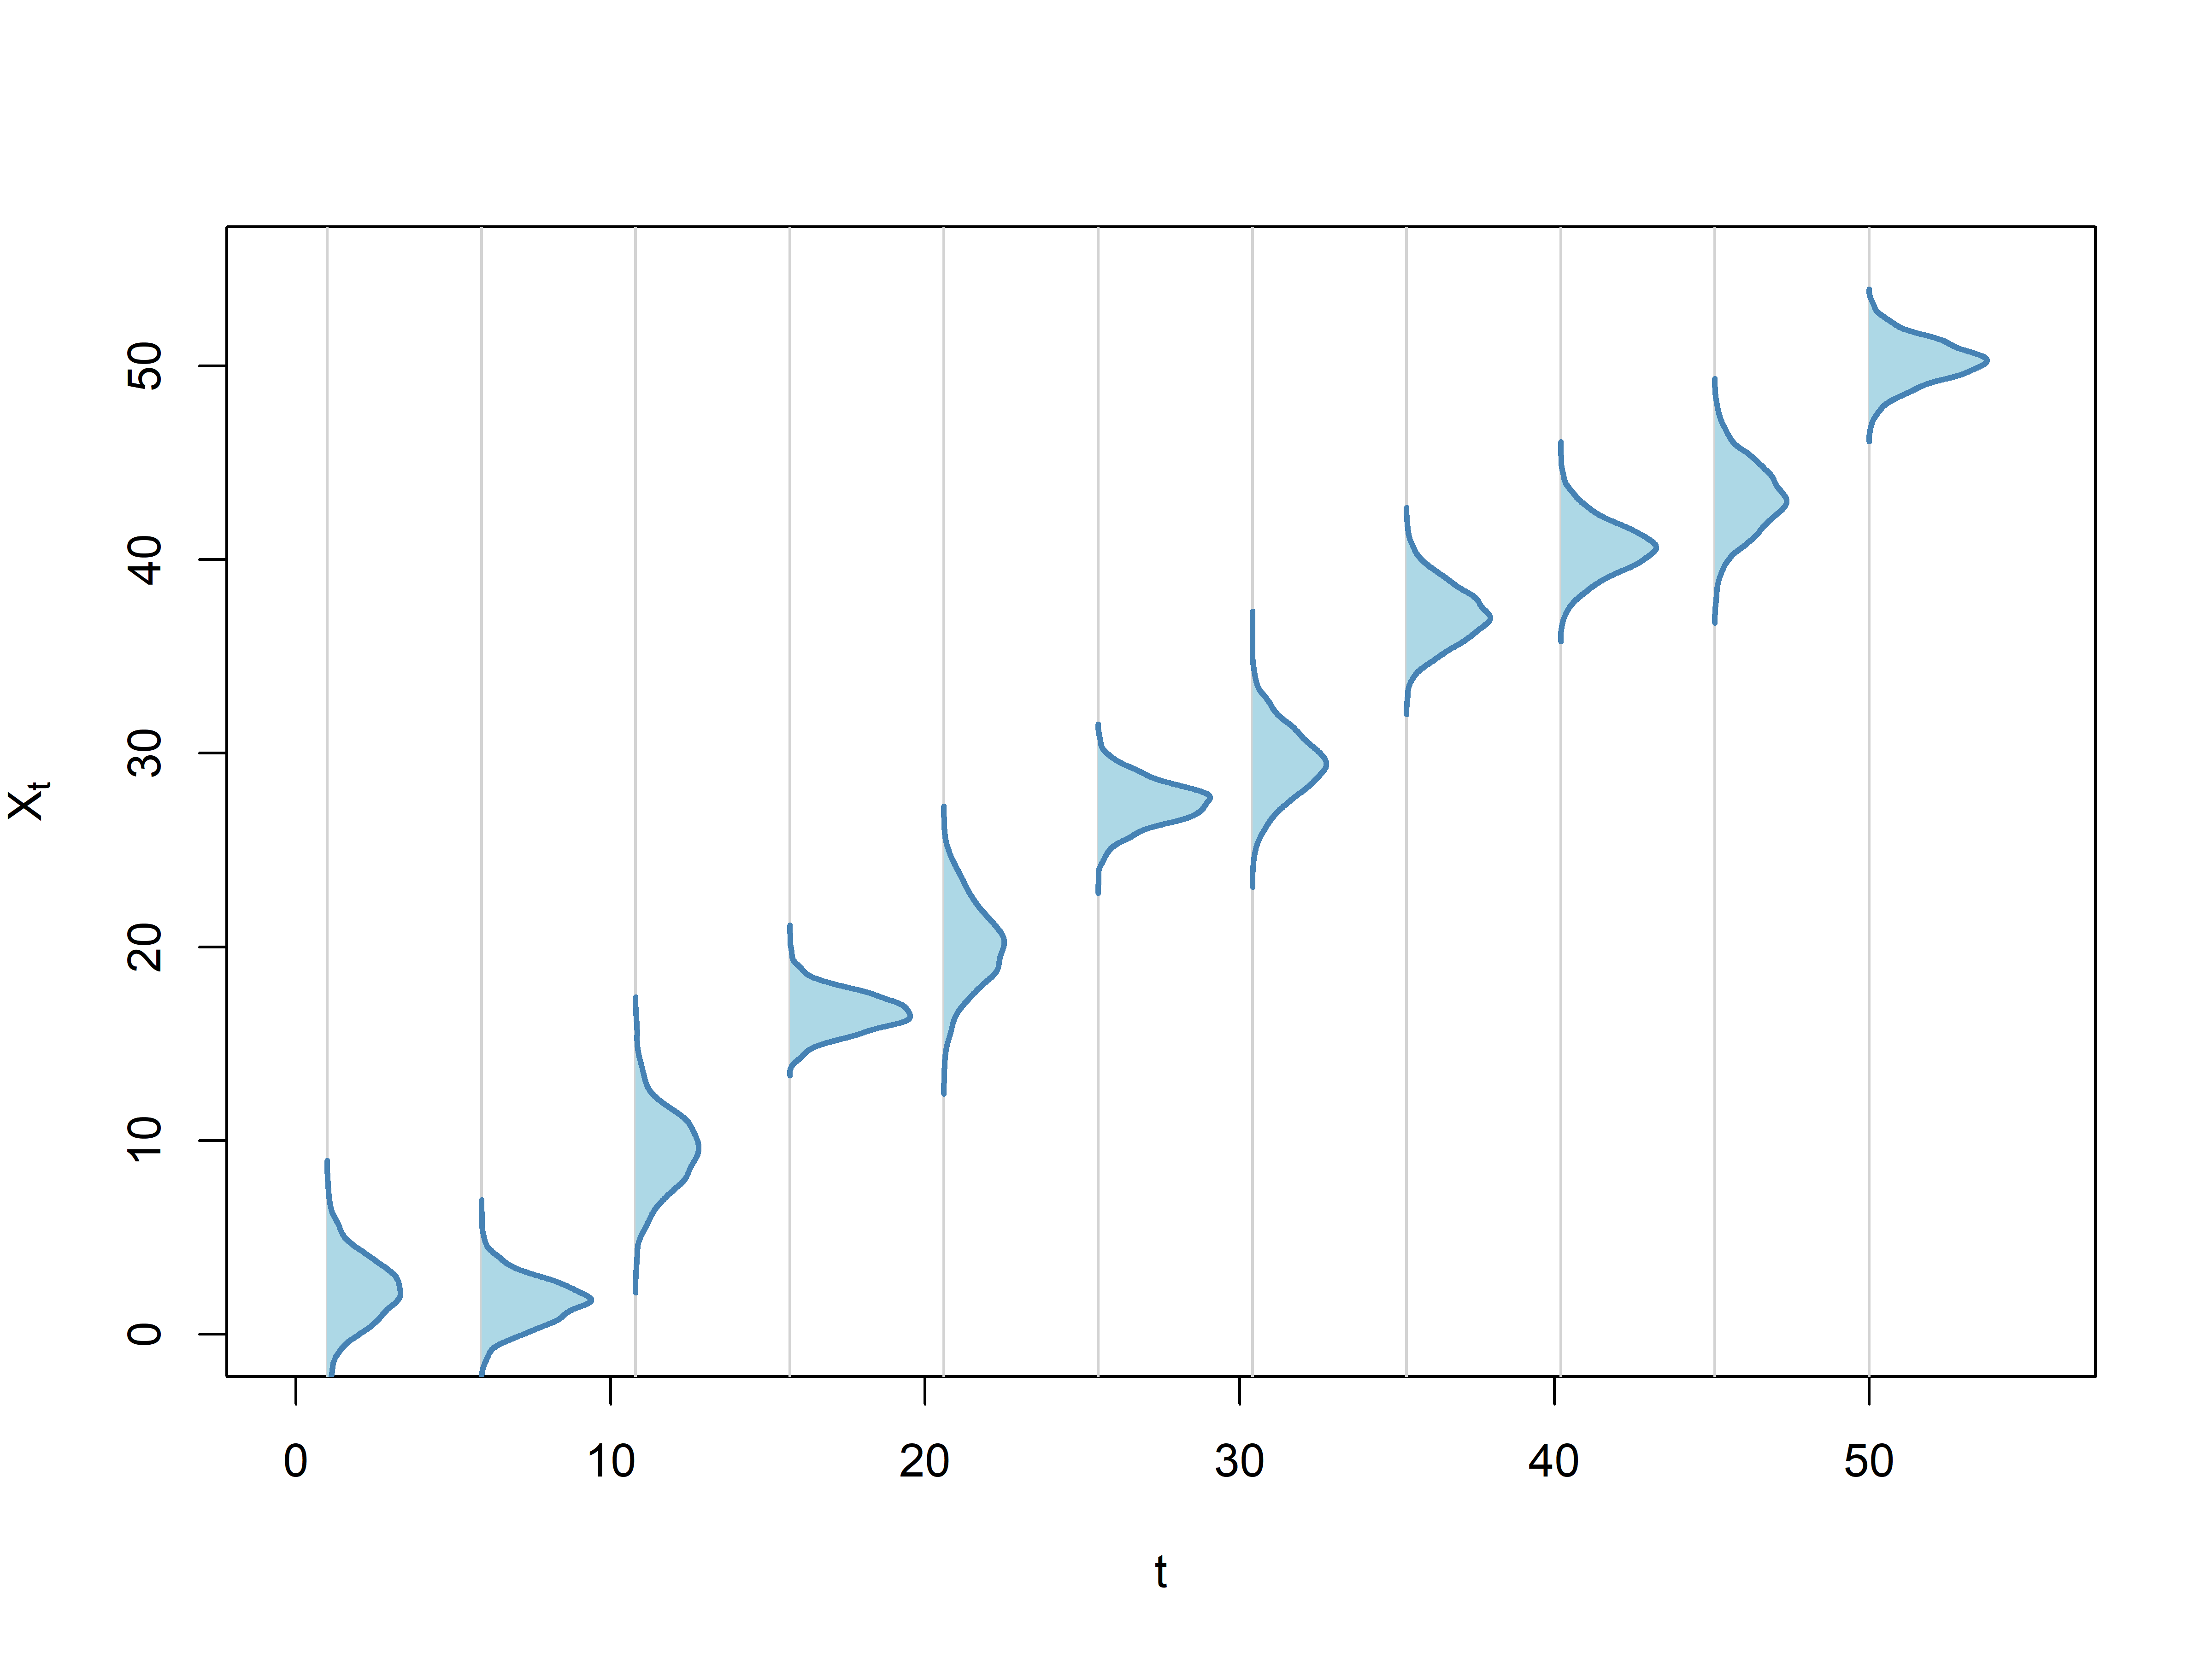
\includegraphics[width=0.48\linewidth]{../img/gp.png}
      \caption{\textit{An example of a Gaussian process on $t \in \{0, \, 10, \, \ldots, \, 50\}$.}}
      \label{figure_1}
   \end{figure}

   \subsection*{Covariance functions}

   ((\hyperref[Roberts2013]{Roberts et al., 2013})) In the following section, we briefly describe commonly used kernels. We start with a simple white noise, and then consider common \textit{stationary} covariances, both uni- and multi-dimensional. We finish this section with periodic and quasi-periodic kernel functions. We note that sums (and products) of valid covariance kernels give valid covariance functions (i.e. the resultant covariance matrices are positive semi-definite) and so we may entertain with ease multiple explanatory hypothesis. 

   \vspace{1em}

   \textit{White noise} with variance $\sigma^2$ is represented by
   
   $$k(x_{i}, \, x_{j}) = \sigma^2\delta_{ij}, \, \text{where} \, \delta_{ij} = 1 \, \text{for} \, i = j \, \text{and} \, \delta_{ij} = 0 \, \text{for} \, i \neq j.$$

   This kernel allows us to entertain uncertainity in our observed data and is so typically found added to other kernels.

   \vspace{1em}

   \textit{The SE kernel} is given by

   $$k(x_{i}, \, x_{j}) = h^{2} \text{exp}(-(\frac{x_i - x_j}{\lambda})^2),$$ 

   where $h$ is an output-scale amplitude and $\lambda$ is an input (length, or time) scale. This gives rather smooth variations with typical time scale of $\lambda$ and admits functions drawn from the GP that are infinitely differentiable.

   \vspace{1em}

   \textit{The rational quadratic (RQ) kernel} is given by

   $$k(x_{i}, \, x_{j}) = h^{2} (1 + \frac{(x_{i} - x_{j})^2}{\alpha\lambda^2})^{-\alpha},$$

   where $\alpha$ is known as the index. ((\hyperref[Rasmussen2006]{Rasmussen and Williams, 2006})) show that this is equivalent to a scale mixture of SE kernels with different length scales, the latter distributed according to a Beta distribution with parameters $\alpha$ and $\lambda^{-2}$. This gives variations with a range of time scales, the distribution peaking around $\lambda$ but extending significantly longer period (but remaining rather smooth). When $\alpha \to \infty$, the RQ kernel reduces to the SE kernel with length scale $\lambda$.

   \vspace{1em}

   \textit{The Mat\'ern} class of covariance functions is defined by

   $$k(x_{i}, \, x_{j}) = h^{2} \frac{1}{\Gamma(v)2^{v-1}} (2\sqrt{v}\frac{|x_{i} - x_{j}|}{\lambda}) \mathbb{B}_{v} (2\sqrt{v}\frac{|x_{i} - x_{j}|}{\lambda}),$$

   where $h$ is the output scale, $\lambda$ is the input scale, $\Gamma()$ is the standard Gamma function and $\mathbb{B}()$ is the modified Bessel function of second order. The additional hyperparameter $v$ controls the degree of differentiability of the resultant functions modelled by a GP with a Mat\'ern covariance function, such that there are only $(v + \frac{1}{2})$ times differentiable. As $v \to \infty$, so the functions become infinitely differentiable and the Matern kernel becomes the SE one. Taking $v = \frac{1}{2}$ gives the exponential kernel

   $$k(x_{i}, \, x_{j}) = h^{2} \text{exp}(-(\frac{x_i - x_j}{\lambda})^2),$$

   which results in functions that are only once differentiable, and corresponds to the Ornstein-Unlenbeck process.

   \subsection*{Prediction}

   ((\hyperref[Betancourt2020]{Betancourt, 2020})) To simulate sampling a function from a Gaussian process and then evaluating the sampled function at the grid of covariate values we can just directly sample from a multivariate normal random number generator.

   \vspace{1em}

   We can also consider \textit{predictions} by taking advantage of the conditional structure of a multivariate normal density function. Consider a grid of observed covariate values $$\{x_{1}^{\text{obs}}, \, \ldots, \, x_{N_{\text{obs}}}^{\text{obs}}\}$$

   where we know the function values $f(x_{n}^{\text{obs}})$, and a grid of unobserved covariate values where we want to predict the functional values, $$\{x_{1}^{\text{pred}}, \, \ldots, \, x_{N_{\text{pred}}}^{\text{pred}}\}.$$

   The parameters of the multivariate normal density function of the combined covariate values decomposes into the parameters of the multivariate normal density function for each component grid plus mixed covariate function evaluations.

   \vspace{1em}

   $\mathbf{m} = 
   \begin{bmatrix}
      m(x_{1}^{\text{obs}}) \\
      \vdots \\
      m(x_{N_{\text{obs}}}^{\text{obs}}) \\
      m(x_{1}^{\text{pred}}) \\
      \vdots \\
      m(x_{N_{\text{pred}}}^{\text{pred}})
   \end{bmatrix}  
   \: 
   \text{and}
   \:
   \mathbf{K} = 
   \begin{bmatrix}
      k(x_{1}^{\text{obs}}, \, x_{1}^{\text{obs}}) 
      & \cdots 
      & k(x_{1}^{\text{obs}}, \, x_{N_{\text{obs}}}^{\text{obs}}) 
      & k(x_{1}^{\text{obs}}, \, x_{1}^{\text{pred}}) 
      & \cdots 
      & k(x_{1}^{\text{obs}}, \, x_{N_{\text{pred}}}^{\text{pred}}) \\
      
      \vdots & \ddots & \vdots & \vdots & \ddots & \vdots \\
      
      k(x_{N_{\text{obs}}}^{\text{obs}}, \, x_{1}^{\text{obs}}) 
      & \cdots 
      & k(x_{N_{\text{obs}}}^{\text{obs}}, \, x_{N_{\text{obs}}}^{\text{obs}}) 
      & k(x_{N_{\text{obs}}}^{\text{obs}}, \, x_{1}^{\text{pred}}) 
      & \cdots 
      & k(x_{N_{\text{obs}}}^{\text{obs}}, \, x_{N_{\text{pred}}}^{\text{pred}}) \\
      
      k(x_{1}^{\text{pred}}, \, x_{1}^{\text{obs}}) 
      & \cdots 
      & k(x_{1}^{\text{pred}}, \, x_{N_{\text{obs}}}^{\text{obs}}) 
      & k(x_{1}^{\text{pred}}, \, x_{1}^{\text{pred}}) 
      & \cdots 
      & k(x_{1}^{\text{pred}}, \, x_{N_{\text{pred}}}^{\text{pred}}) \\
      
      \vdots & \ddots & \vdots & \vdots & \ddots & \vdots \\
      
      k(x_{N_{\text{pred}}}^{\text{pred}}, \, x_{1}^{\text{obs}}) 
      & \cdots 
      & k(x_{N_{\text{pred}}}^{\text{pred}}, \, x_{N_{\text{obs}}}^{\text{obs}}) 
      & k(x_{N_{\text{pred}}}^{\text{pred}}, \, x_{1}^{\text{pred}}) 
      & \cdots 
      & k(x_{N_{\text{pred}}}^{\text{pred}}, \, x_{N_{\text{pred}}}^{\text{pred}})
   \end{bmatrix}$,

   \vspace{1em}
   
   more compactly,

   \vspace{1em}

   $$\mathbf{m} = 
   \begin{bmatrix}
      \mathbf{m}_{\text{obs}} \\
      \\
      \mathbf{m}_{\text{pred}}
   \end{bmatrix}  
   \: 
   \text{and}
   \:
   \mathbf{K} = 
   \begin{bmatrix}
      \mathbf{K}_{\text{obs}} & \mathbf{K}_{\text{mix}} \\
      \\
      (\mathbf{K}_{\text{mix}})^{\text{T}} & \mathbf{K}_{\text{pred}}
   \end{bmatrix}$$.

   \vspace{1em}

   The conditional probability density function for the unobserved function values $(f_{\text{pred}})_{n} = f(x_{n}^{\text{pred}})$ given the observed function values  $(f_{\text{obs}})_{n} = f(x_{n}^{\text{obs}})$ falls into the multivariate normal family,

   $$\pi(\mathbf{f}_{\text{pred}} | \mathbf{f}_{\text{obs}}) \sim \mathcal{N}_{n}(\boldsymbol{\mu}, \boldsymbol{\Sigma})$$

   with the location parameters 

   $$\boldsymbol{\mu} = \mathbf{m}_{\text{pred}} + (\mathbf{K}_{\text{mix}})^{\text{T}} \cdot (\mathbf{K}_{\text{obs}})^{-1} \cdot (\mathbf{f}_{\text{obs}} - \mathbf{m}_{\text{obs}}) $$

   and the covariance matrix parameters

   $$\boldsymbol{\Sigma} = \mathbf{K}_{\text{pred}} - (\mathbf{K}_{\text{mix}})^{\text{T}} \cdot (\mathbf{K}_{\text{obs}})^{-1} \cdot \mathbf{K}_{\text{mix}}.$$

   Inference with Gaussian process priors proceeds similarly. Once we've identified the covariate values at which we have observations or will want to make predictions we can specify the marginalized prior model with the corresponding multivariate normal density function. If the observational model is normal then we can generate predictions analytically with the conditioning operations for the posterior covariance function.

   \section*{Air pollution example}
   \subsection*{Exploratory data analysis}
   
      \begin{table}[H]
         \centering
         \begin{tabularx}{\textwidth}{|l|l|X|l|}
         \hline
         \text{Variable} & \text{Name} & \text{Description} & \text{Unit} \\
         \hline
         \(\text{NO}_{2}\) & Nitrogen dioxide & A harmful gas from vehicles and industry. & \(\mu\text{g}/\text{m}^{3}\) \\
         \(\text{PM}_{10}\) & Particulate matter 10 & Small inhalable dust particles. & \(\mu\text{g}/\text{m}^{3}\) \\
         \(\text{SO}_{2}\) & Sulphur dioxide & Mainly from burning fossil fuels. & \(\mu\text{g}/\text{m}^{3}\) \\
         Speed & Wind speed & How fast the wind is moving. & m/s \\
         \hline
         \end{tabularx}
         \caption{\textit{Description of variables of the air pollution dataset.}}
         \label{tab:variable_description}
      \end{table}

      \begin{table}[H]
         \centering
         \begin{tabularx}{\textwidth}{|l|X|X|X|X|X|X|X|X|}
            \hline
            Variable & Min. & 1st Qu. & Median & Mean & Std. & 3rd Qu. & Max. & NA's \\
            \hline
            NO$_2$   & 0.0 & 5.0  & 9.0  & 12.73 & 10.72 & 17.0 & 113.0 & 734 \\
            PM$_{10}$ & 0.0 & 12.0 & 17.0 & 19.82 & 12.30 & 24.0 & 158.0 & 298 \\
            SO$_2$   & 0.0 & 2.0  & 3.0  & 6.20  & 11.30 & 5.0  & 142.0 & 638 \\
            Speed    & 0.5 & 2.3  & 3.6  & 3.74  & 1.71  & 4.9  & 11.2  & 918 \\
            \hline
         \end{tabularx}
         \caption{\textit{Summary statistics of the air pollution dataset.}}
         \label{tab:summary_statistics}
      \end{table}

      \begin{figure}[H]
         \centering
         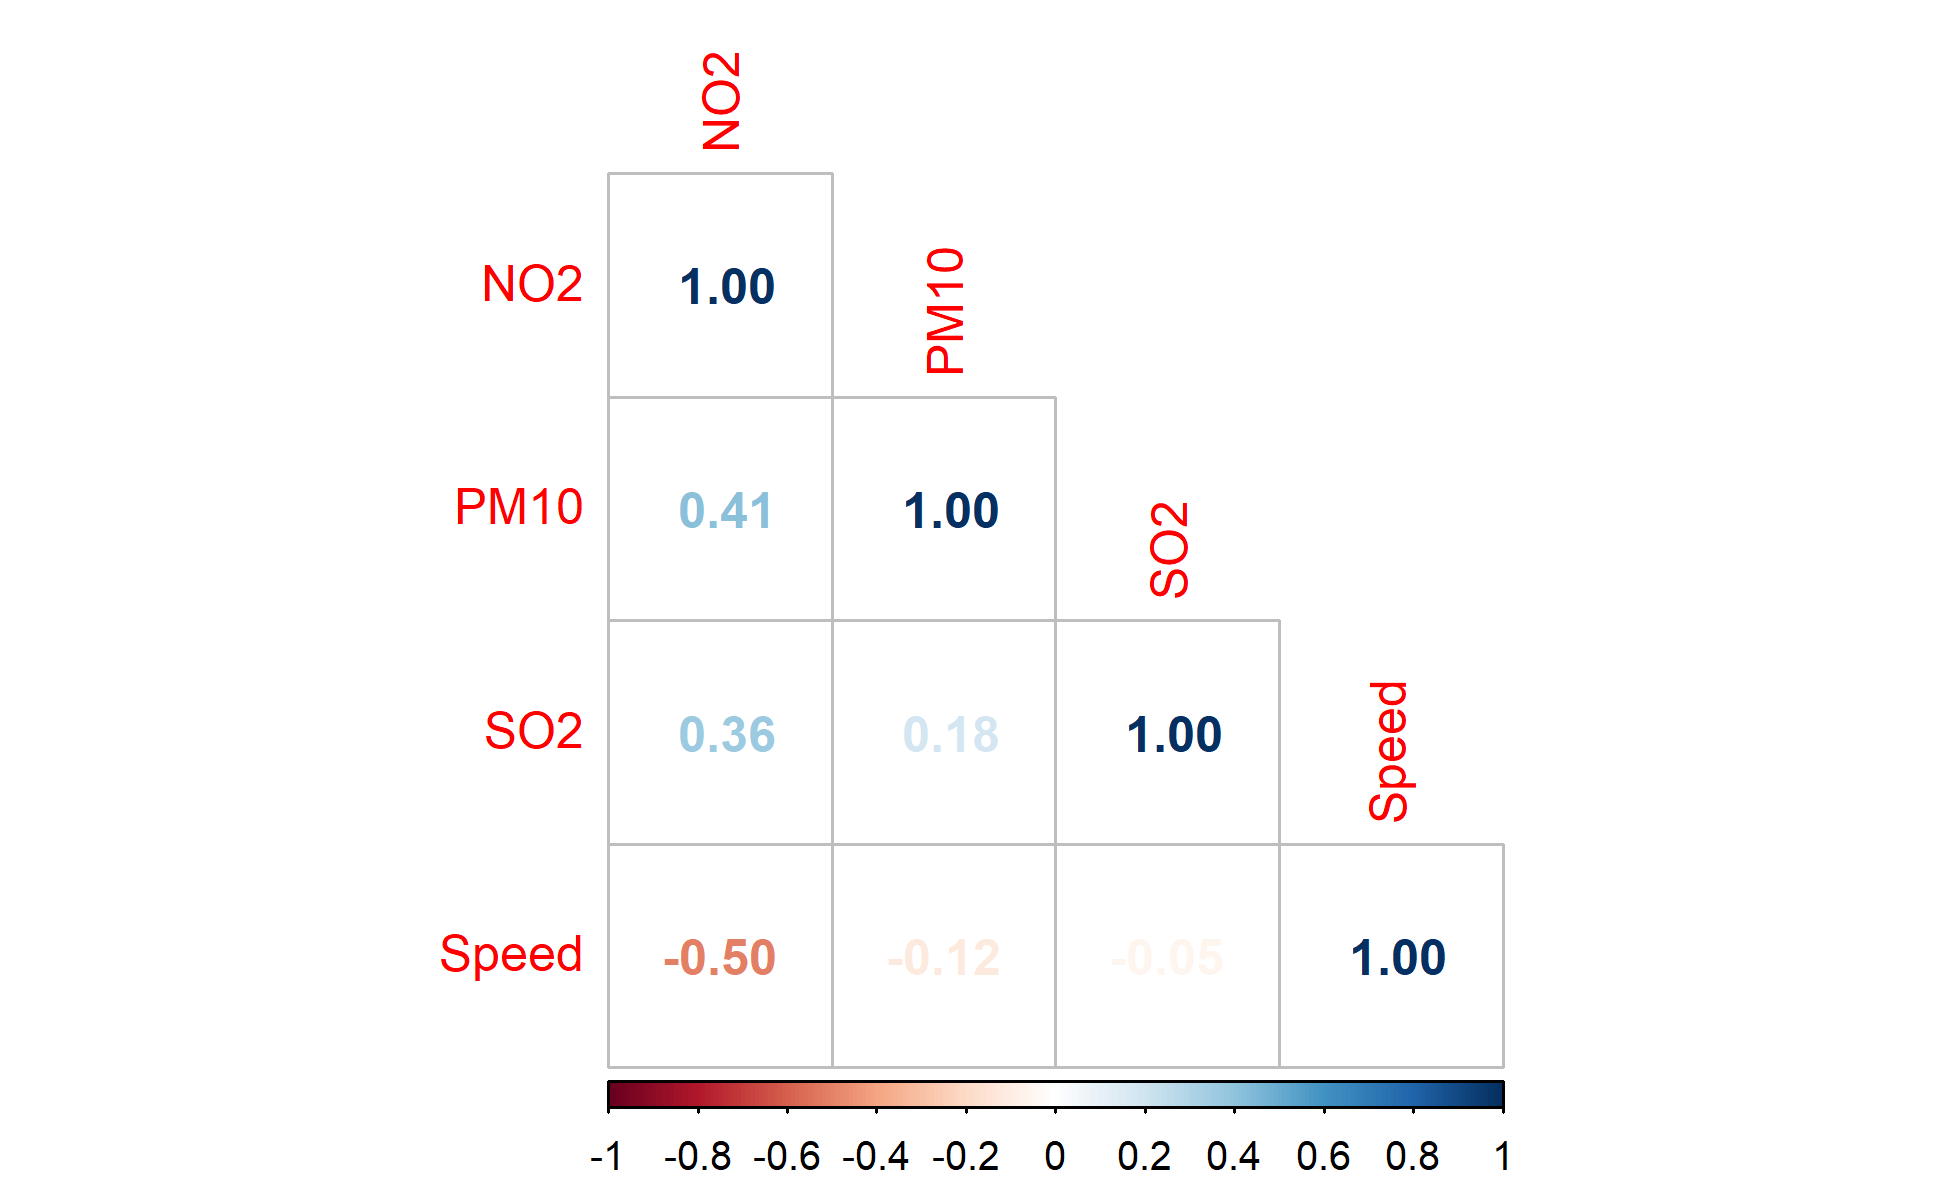
\includegraphics[width=0.48\linewidth]{../img/corrplot.png}
         \caption{\textit{Correlation plot of the air pollution dataset.}}
      \end{figure}

      Our response variable $\text{NO}_{2}$ appears to be moderately positively correlated with $\text{PM}_{10}$ and $\text{SO}_{2}$, and moderately negatively correlated with Speed. These are not ideal explanatory variables since we typically would like them to be strongly correlated with the response variable. The explanatory variables are weekly correlated with one another, whether it be positive or negative correlation. This is ideal since some models do not work well with correlated explanatory variables, often leading to unstable point estimates and inflated standard errors.

      \begin{figure}[H]
         \centering
         \begin{subfigure}{0.48\linewidth}
            \centering
            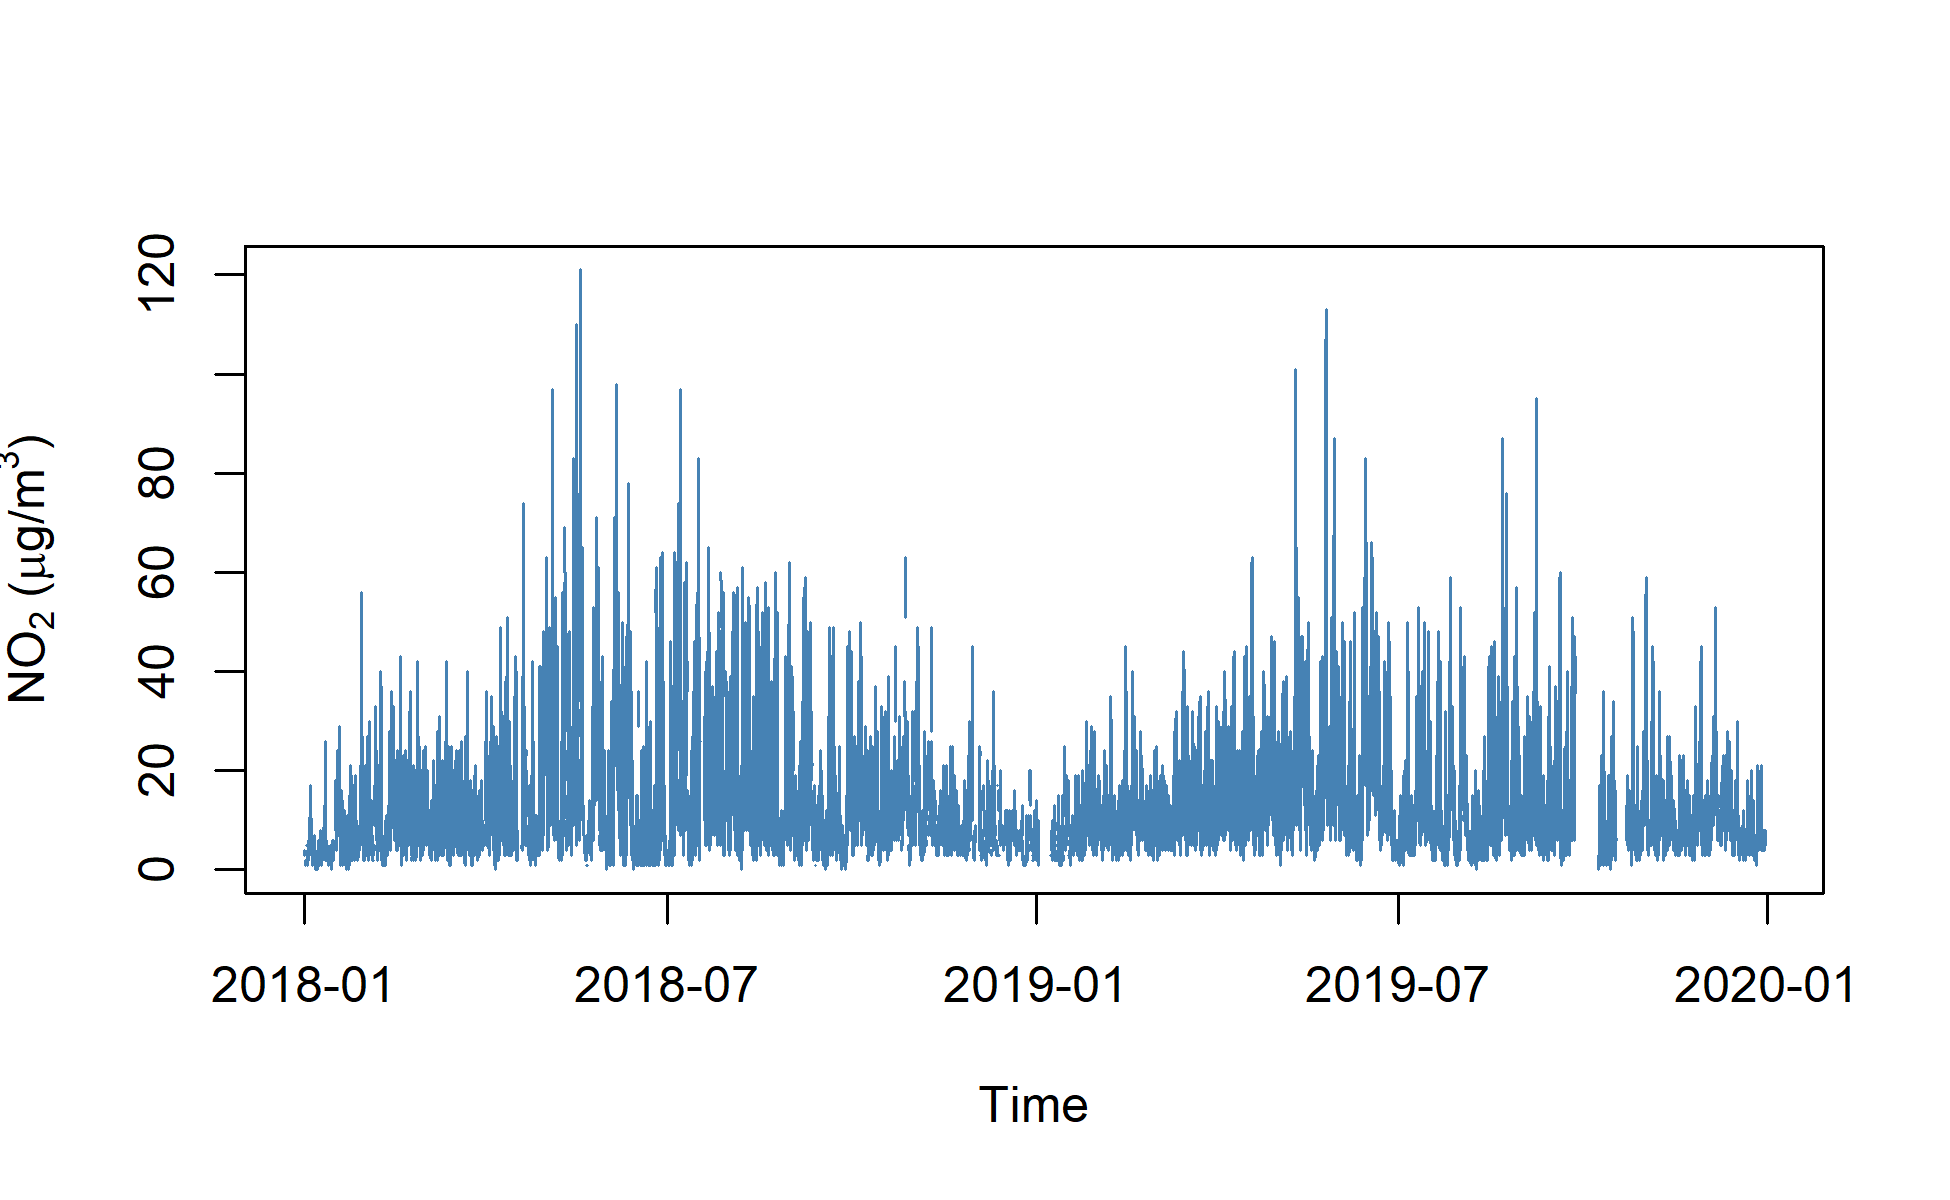
\includegraphics[width=\linewidth]{../img/extracted_no2.png}
         \caption{Nitrogen dioxide}
         \end{subfigure}
         \hfill
         \begin{subfigure}{0.48\linewidth}
            \centering
            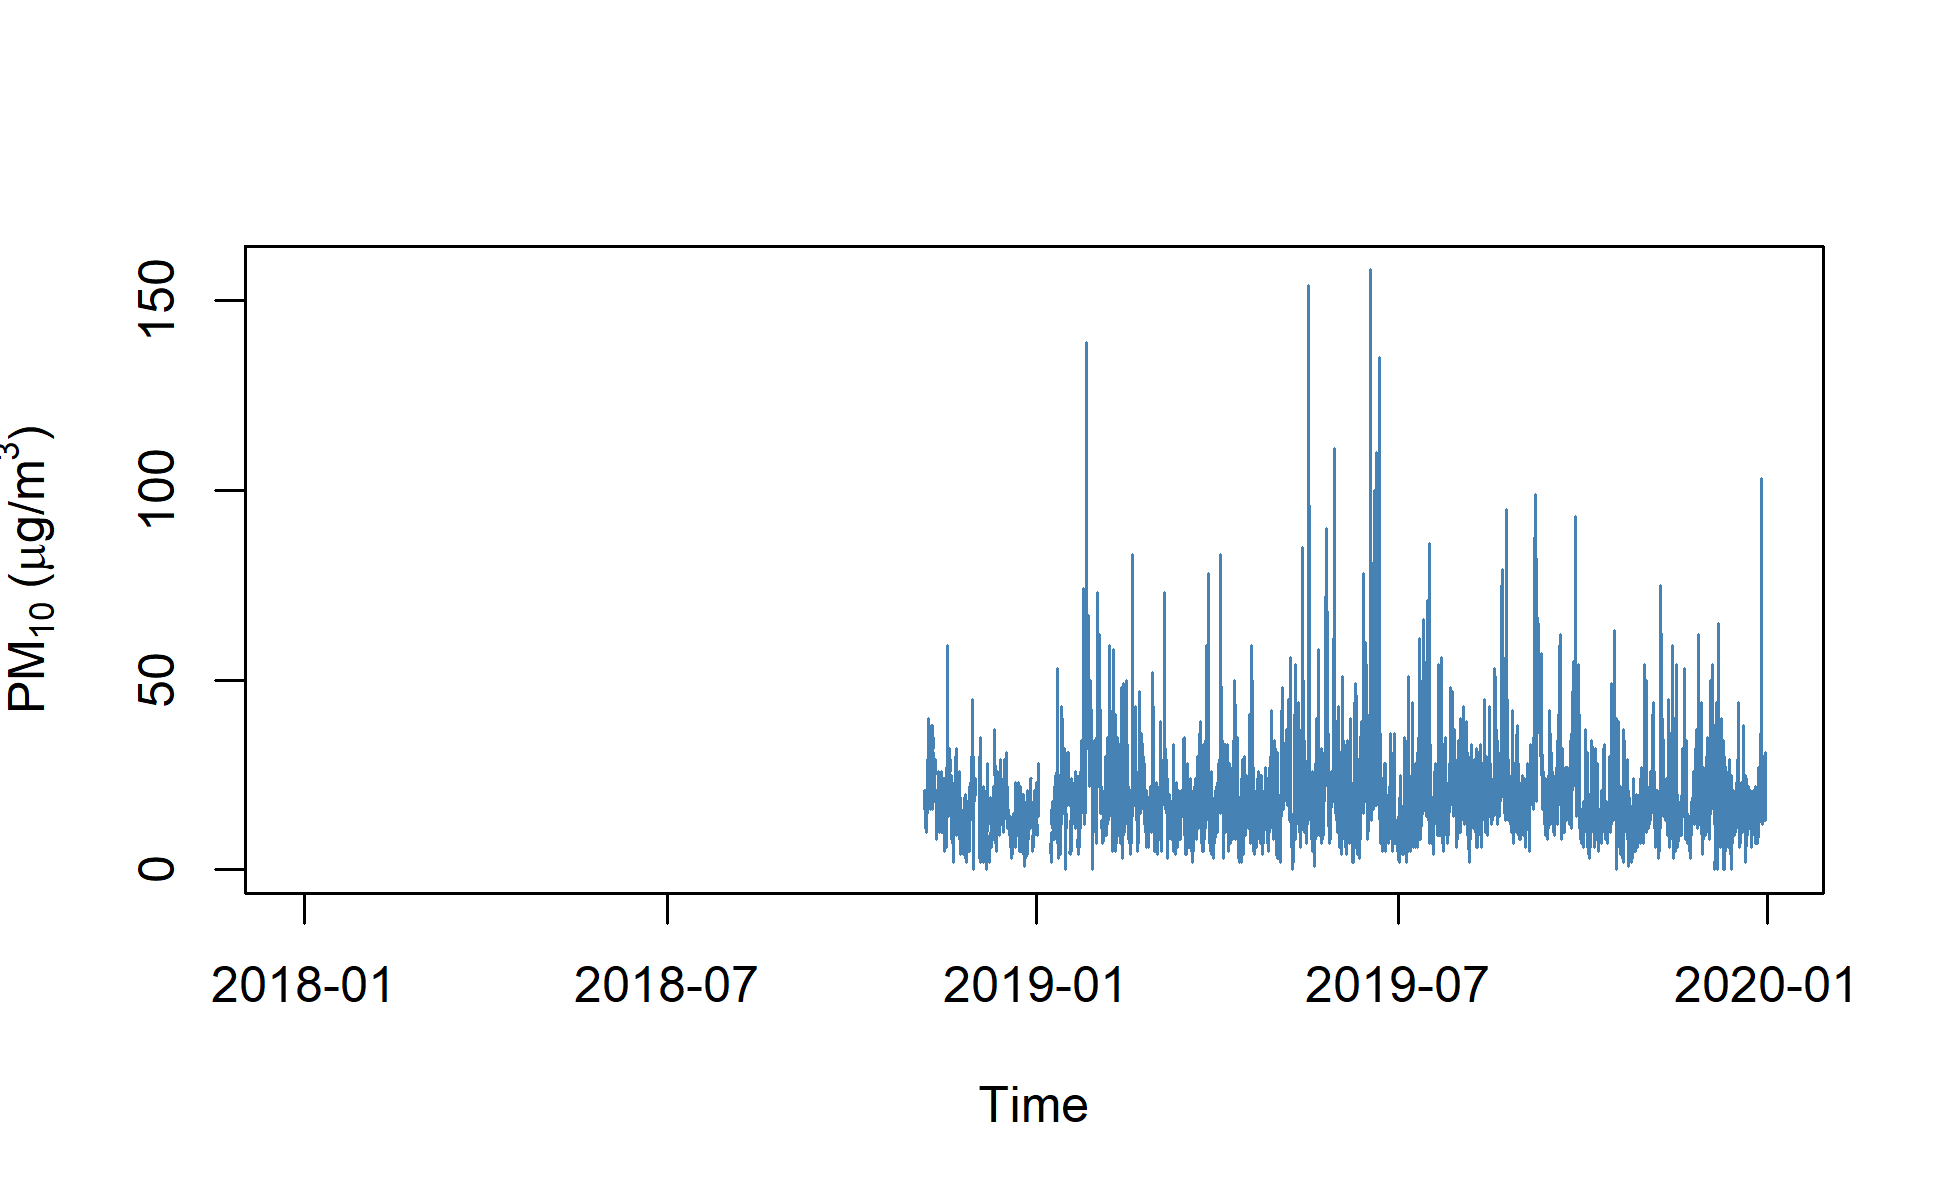
\includegraphics[width=\linewidth]{../img/extracted_pm10.png}
            \caption{Particulate matter 10}
         \end{subfigure}
         
         \vspace{0.5em}

         \begin{subfigure}{0.48\linewidth}
            \centering
            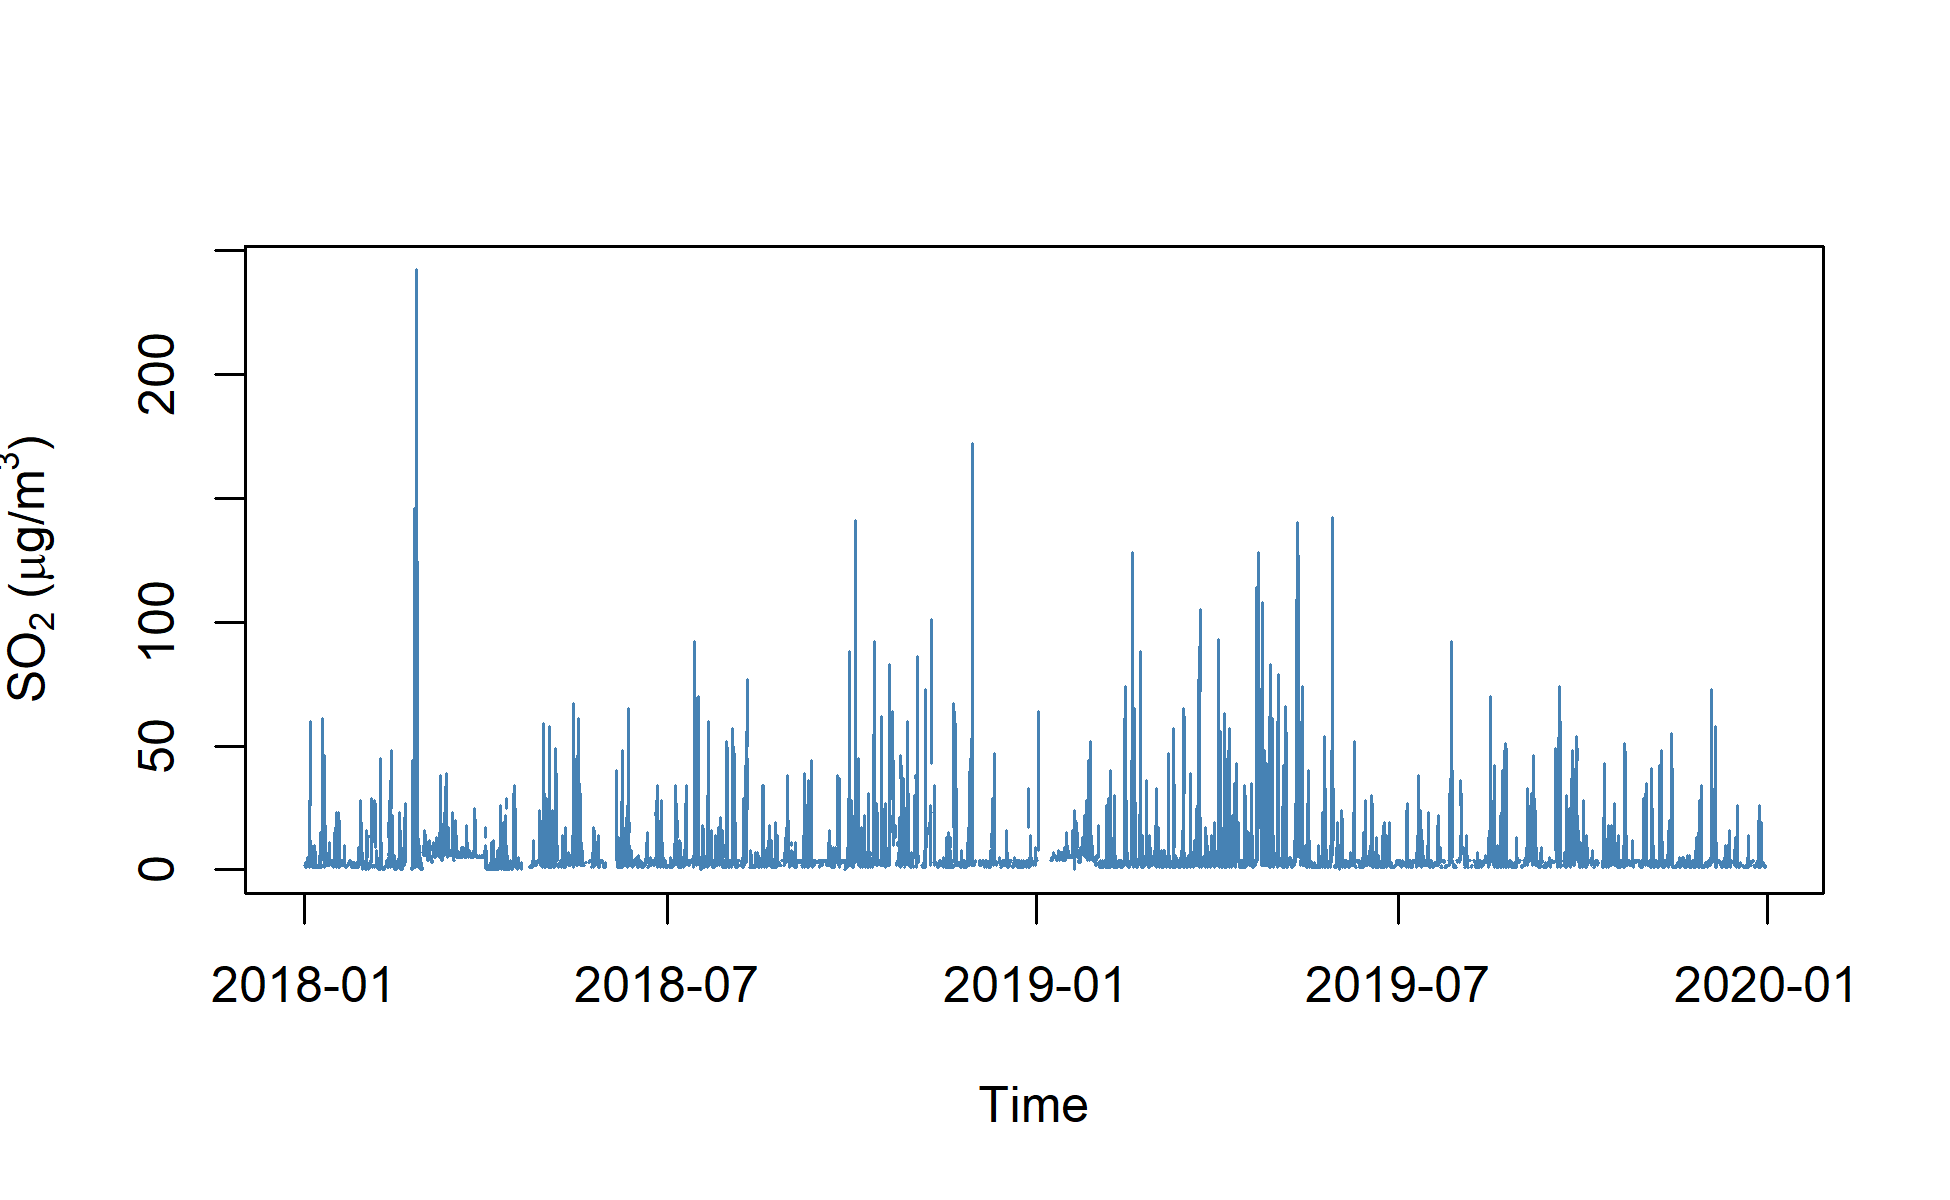
\includegraphics[width=\linewidth]{../img/extracted_so2.png}
         \caption{Sulphur dioxide}
         \end{subfigure}
         \hfill
         \begin{subfigure}{0.48\linewidth}
            \centering
            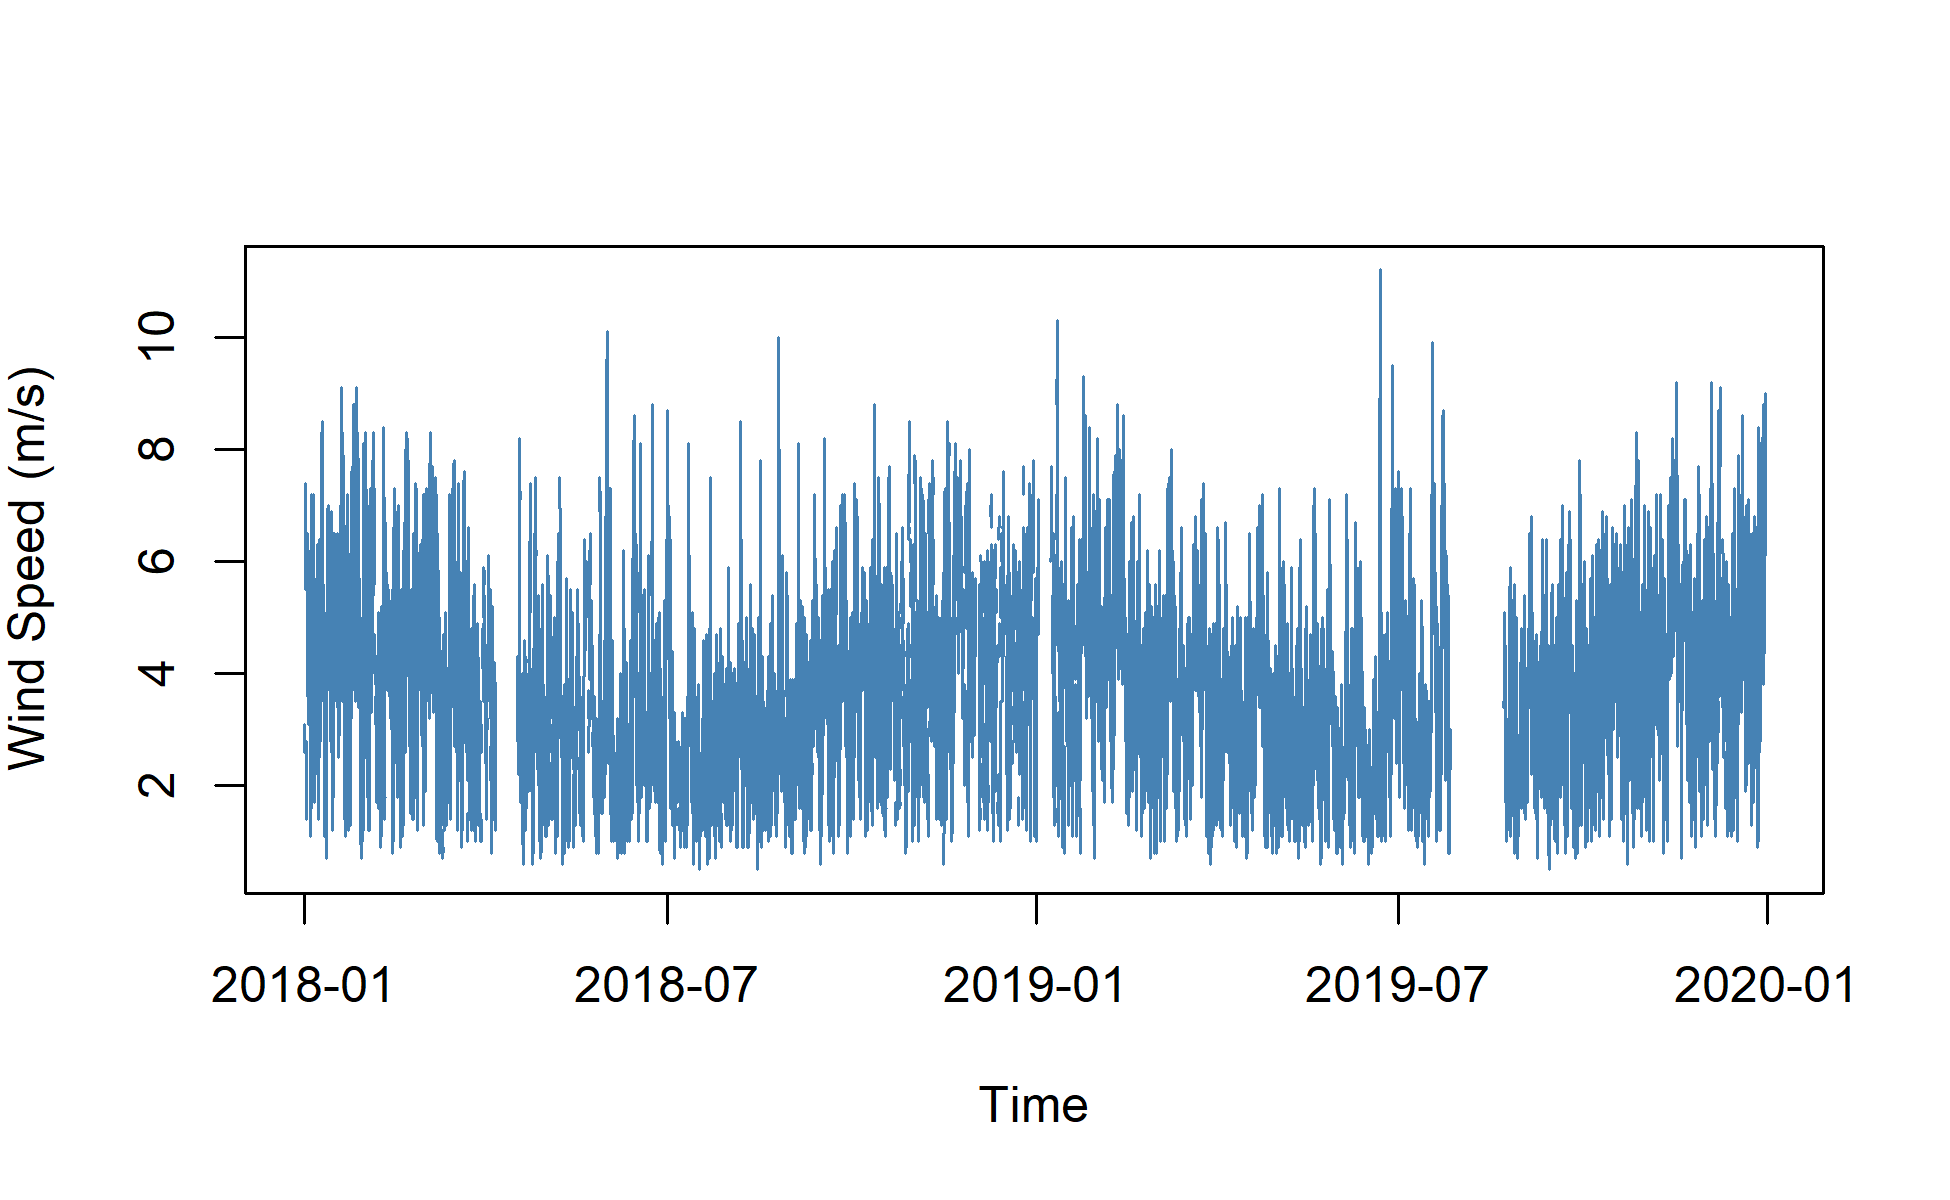
\includegraphics[width=\linewidth]{../img/extracted_speed.png}
            \caption{Wind speed}
         \end{subfigure}

         \caption{\textit{Time-series plots of nitrogen dioxide and mereorological processes from 01/01/2018 to 31/12/2019 measured hourly. Similar cyclic patterns can be observed in the meteorological processes, and a weaker seasonality component can be noted in the yearly nitrogen dioxide processes.}}
      \end{figure}

      \begin{figure}[H]
         \centering
         \begin{subfigure}{0.48\linewidth}
            \centering
            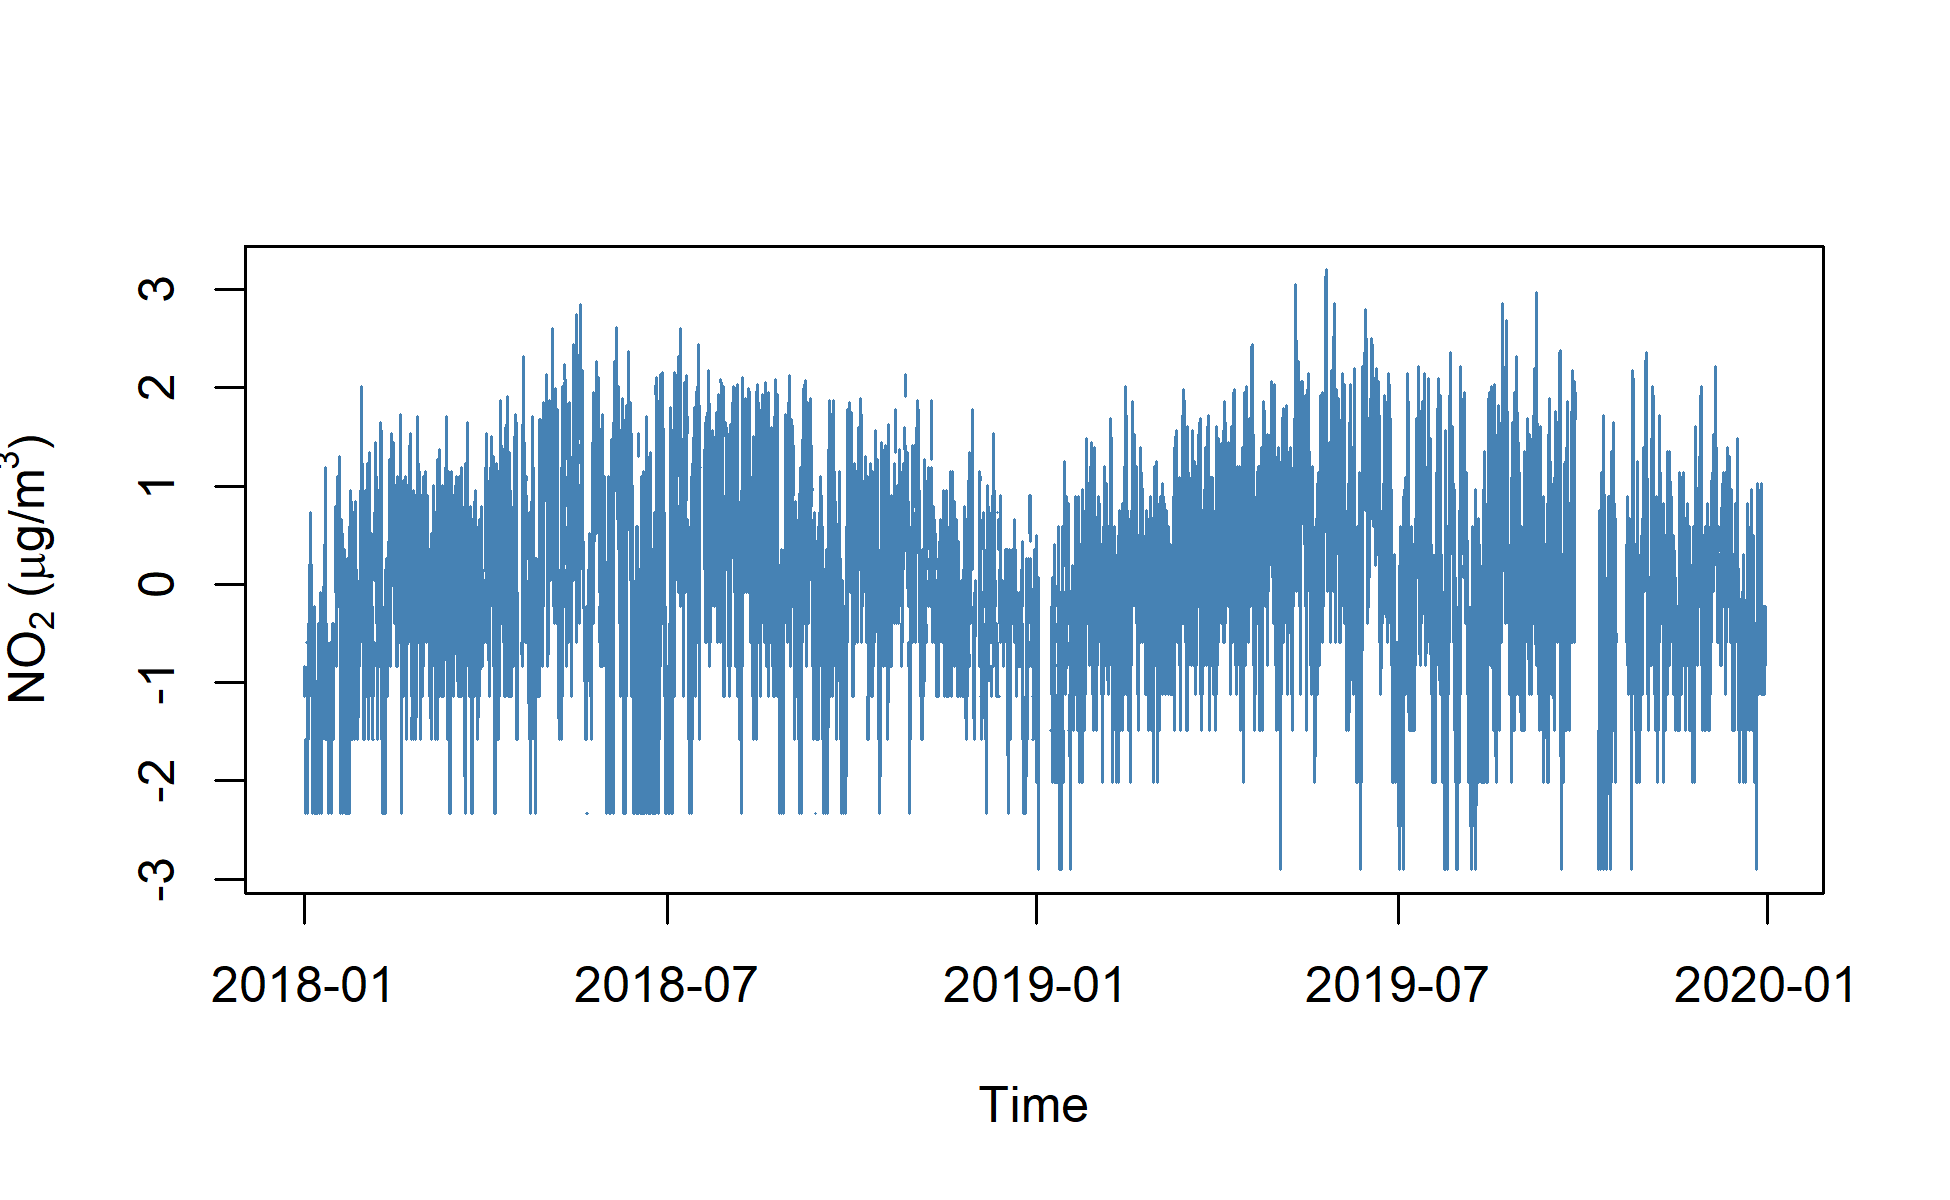
\includegraphics[width=\linewidth]{../img/transformed_no2.png}
         \caption{Nitrogen dioxide}
         \end{subfigure}
         \hfill
         \begin{subfigure}{0.48\linewidth}
            \centering
            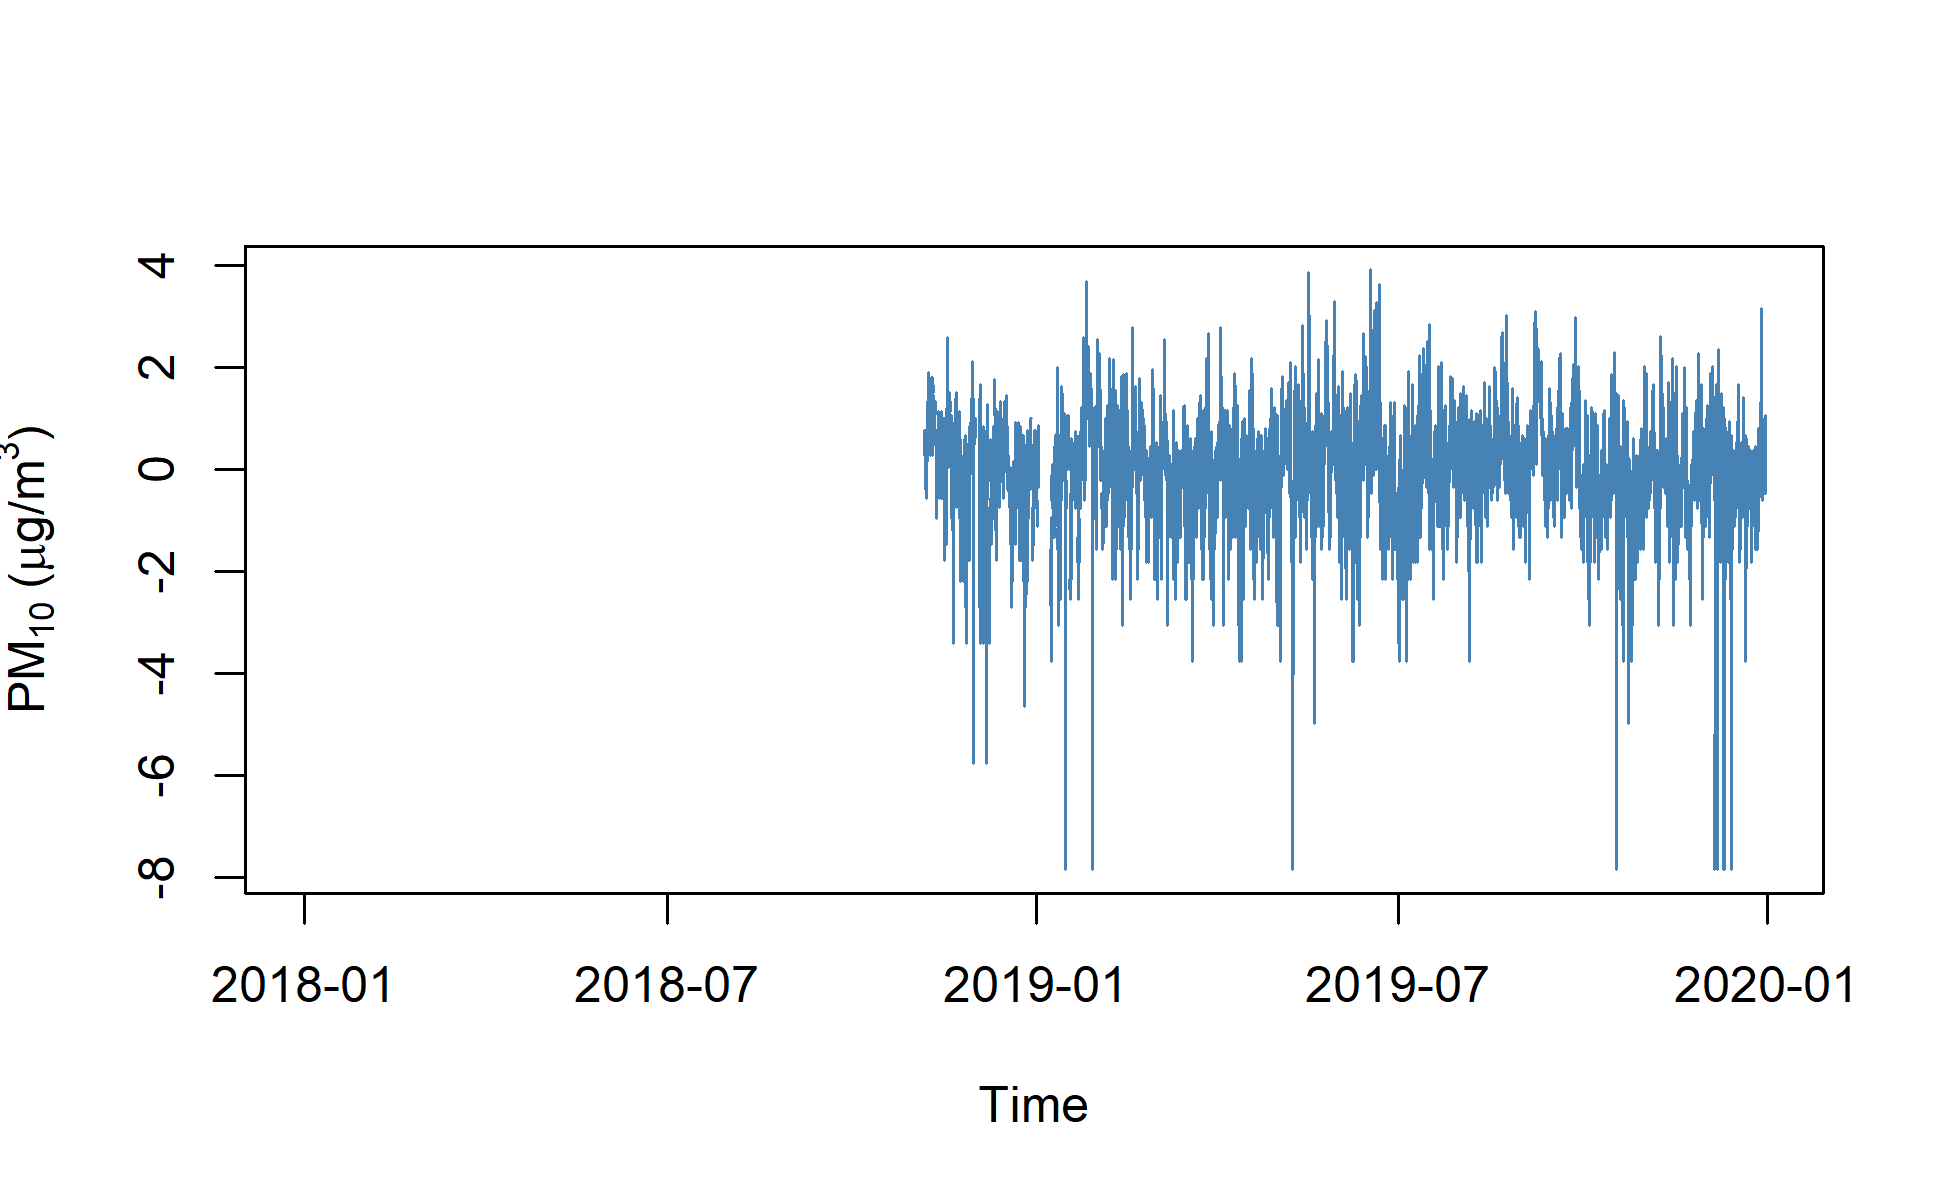
\includegraphics[width=\linewidth]{../img/transformed_pm10.png}
            \caption{Particulate matter 10}
         \end{subfigure}
         
         \vspace{0.5em}

         \begin{subfigure}{0.48\linewidth}
            \centering
            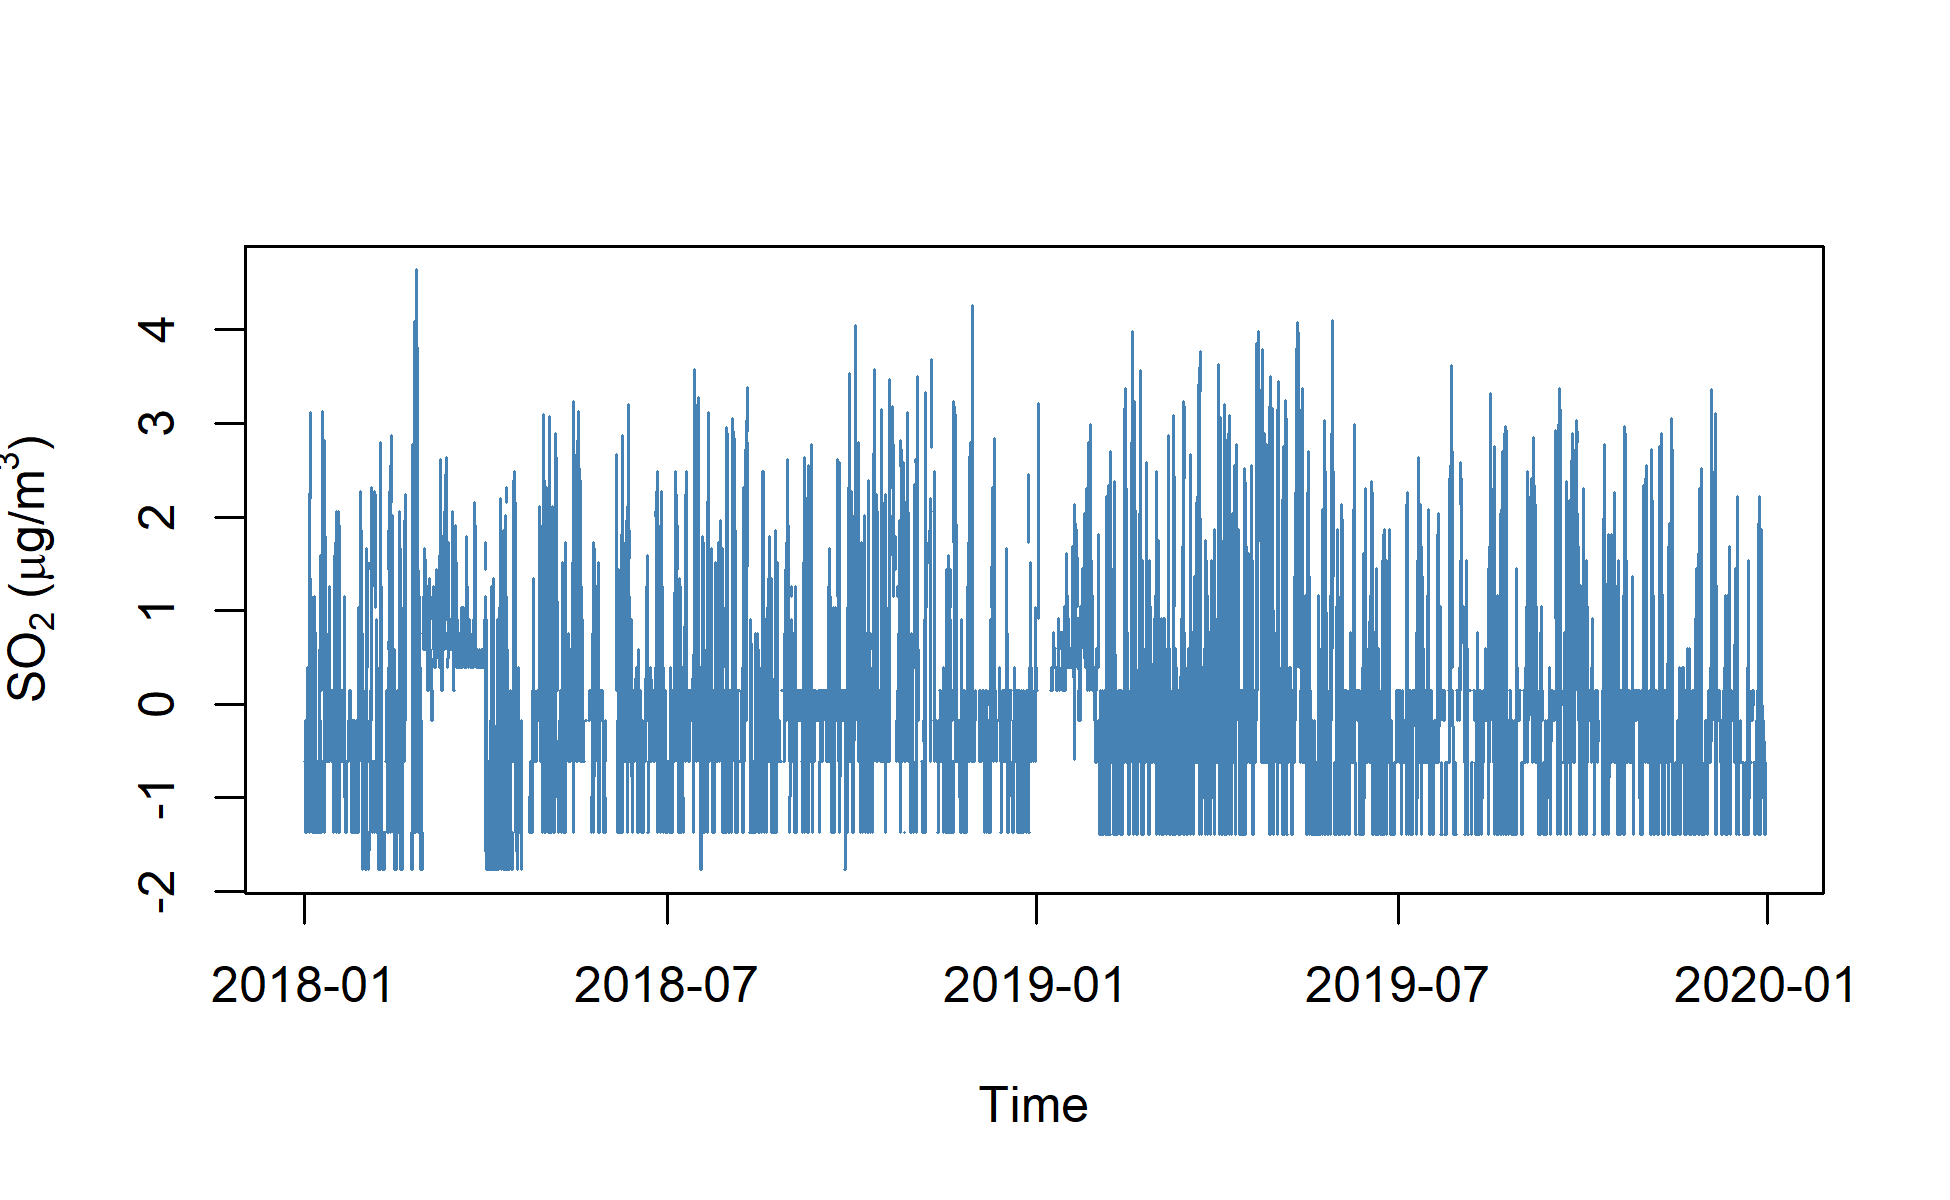
\includegraphics[width=\linewidth]{../img/transformed_so2.png}
         \caption{Sulphur dioxide}
         \end{subfigure}
         \hfill
         \begin{subfigure}{0.48\linewidth}
            \centering
            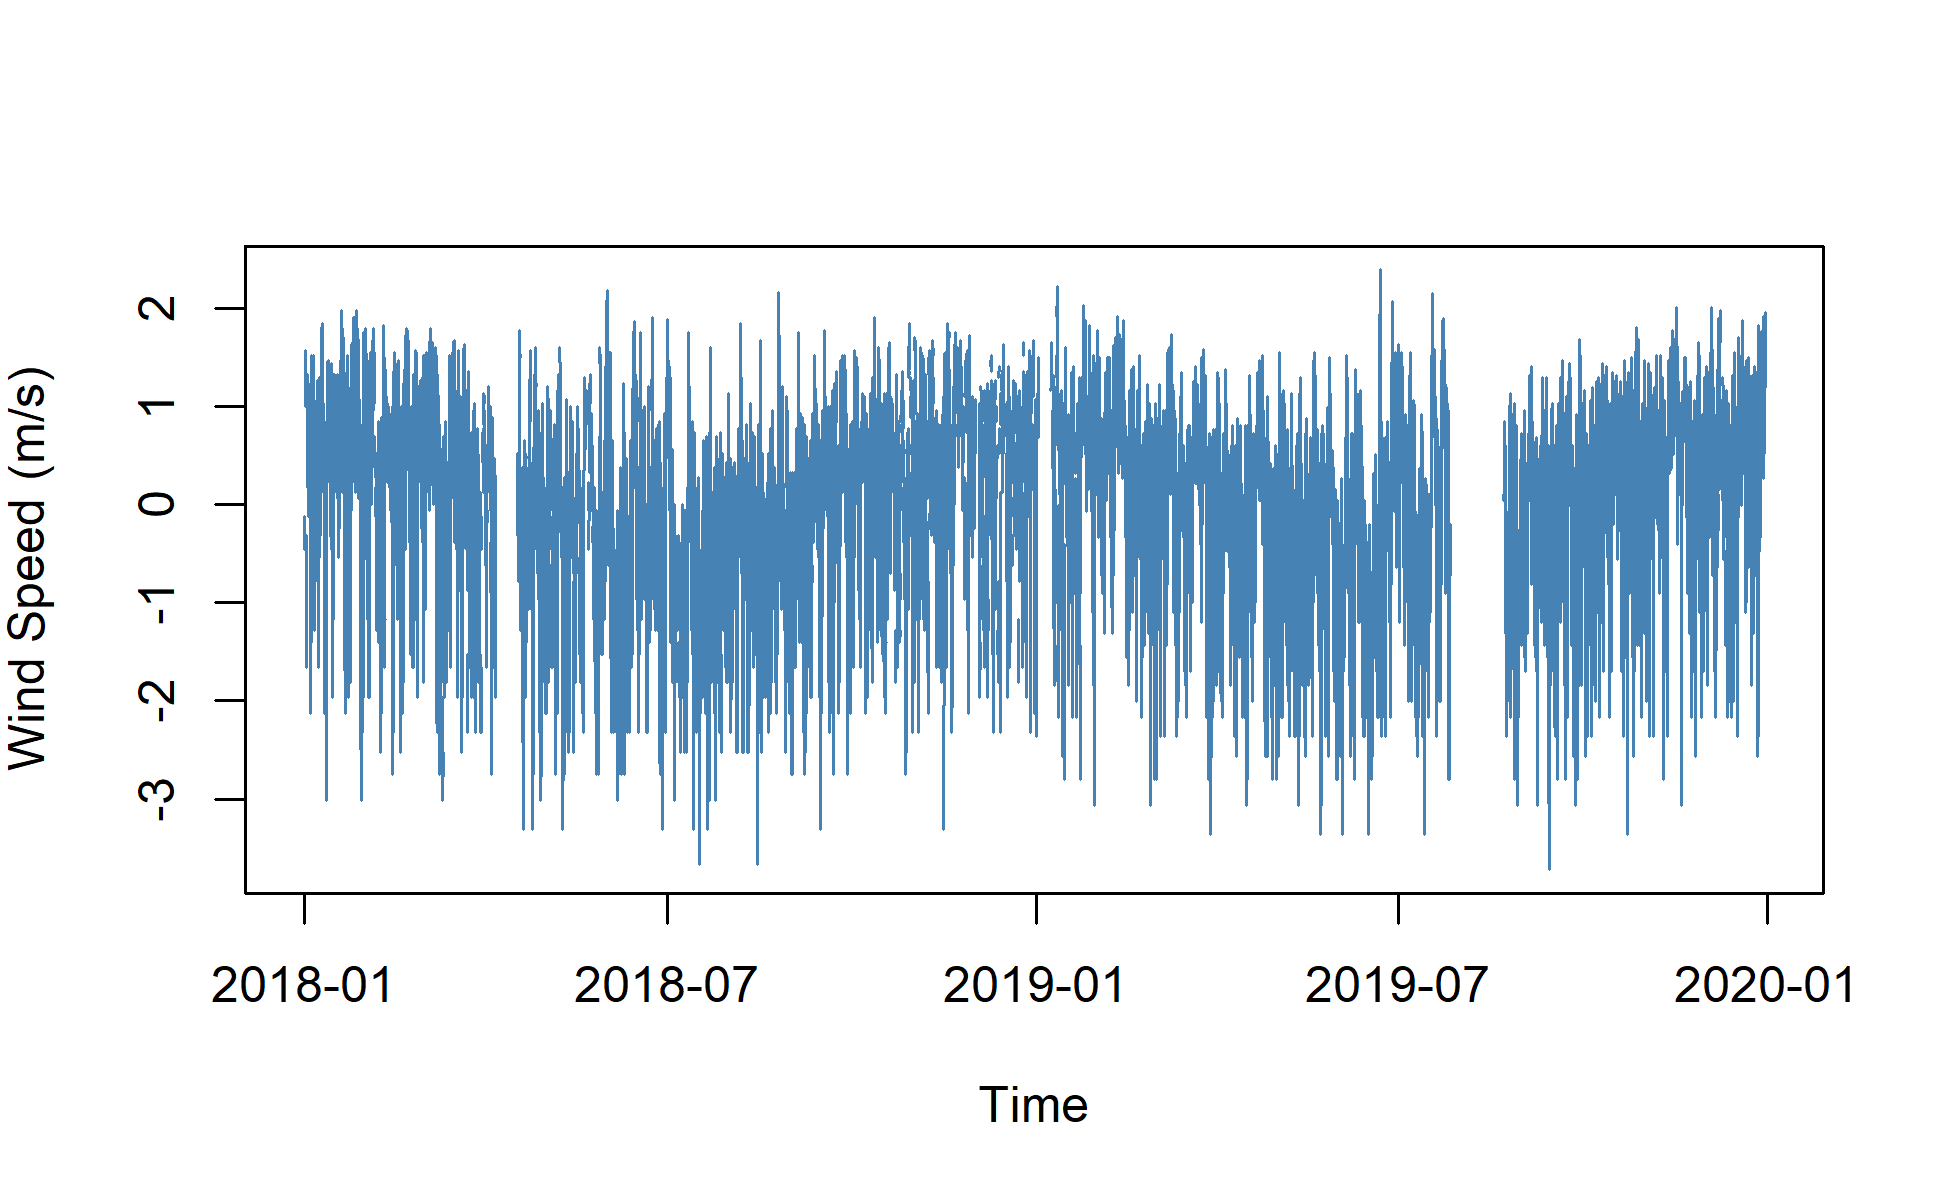
\includegraphics[width=\linewidth]{../img/transformed_speed.png}
            \caption{Wind speed}
         \end{subfigure}

         \caption{\textit{Post-processed daily curves of the nitrogen dioxide and meteorological data, both standardized by their overall mean and standard deviation.}}
      \end{figure}

      \subsection*{Components of the time series}     

      The response variable time-series $x_{t}$ is not statationary because the mean and variance are changing with time. To achieve stationarity there is a need for detrending and a variance stabilizing transformation. In order to stabilize the variance we use Box-Cox transformations in the training set, $y_{t} = (x_{t}^{\lambda} - 1) / \lambda$. The Box-Cox transformations allow us to experiment with a wide variety of $\lambda$ values. A good value of $\lambda$ is one the makes the variation in the data constant through time (Neil Watson, 2024). The \texttt{R} package \texttt{forecast} was used to perform the Box-Cox transformation which yielded an optimal value of $\hat{\lambda} \approx 0$, suggesting a logarithmic transformation. Then, conducting first-order differencing at lag one to remove the trend $z_{t} = y_{t} - y_{t-1} \, \text{for} \, t \in \{2, \, 3, \, \ldots, \, p\}$. The time series $z_{t}$ is now stationary. Thus, we only need to account for the mean and variance in our models.      

      \begin{figure}[H]
         \centering
         \begin{subfigure}{0.48\linewidth}
            \centering
            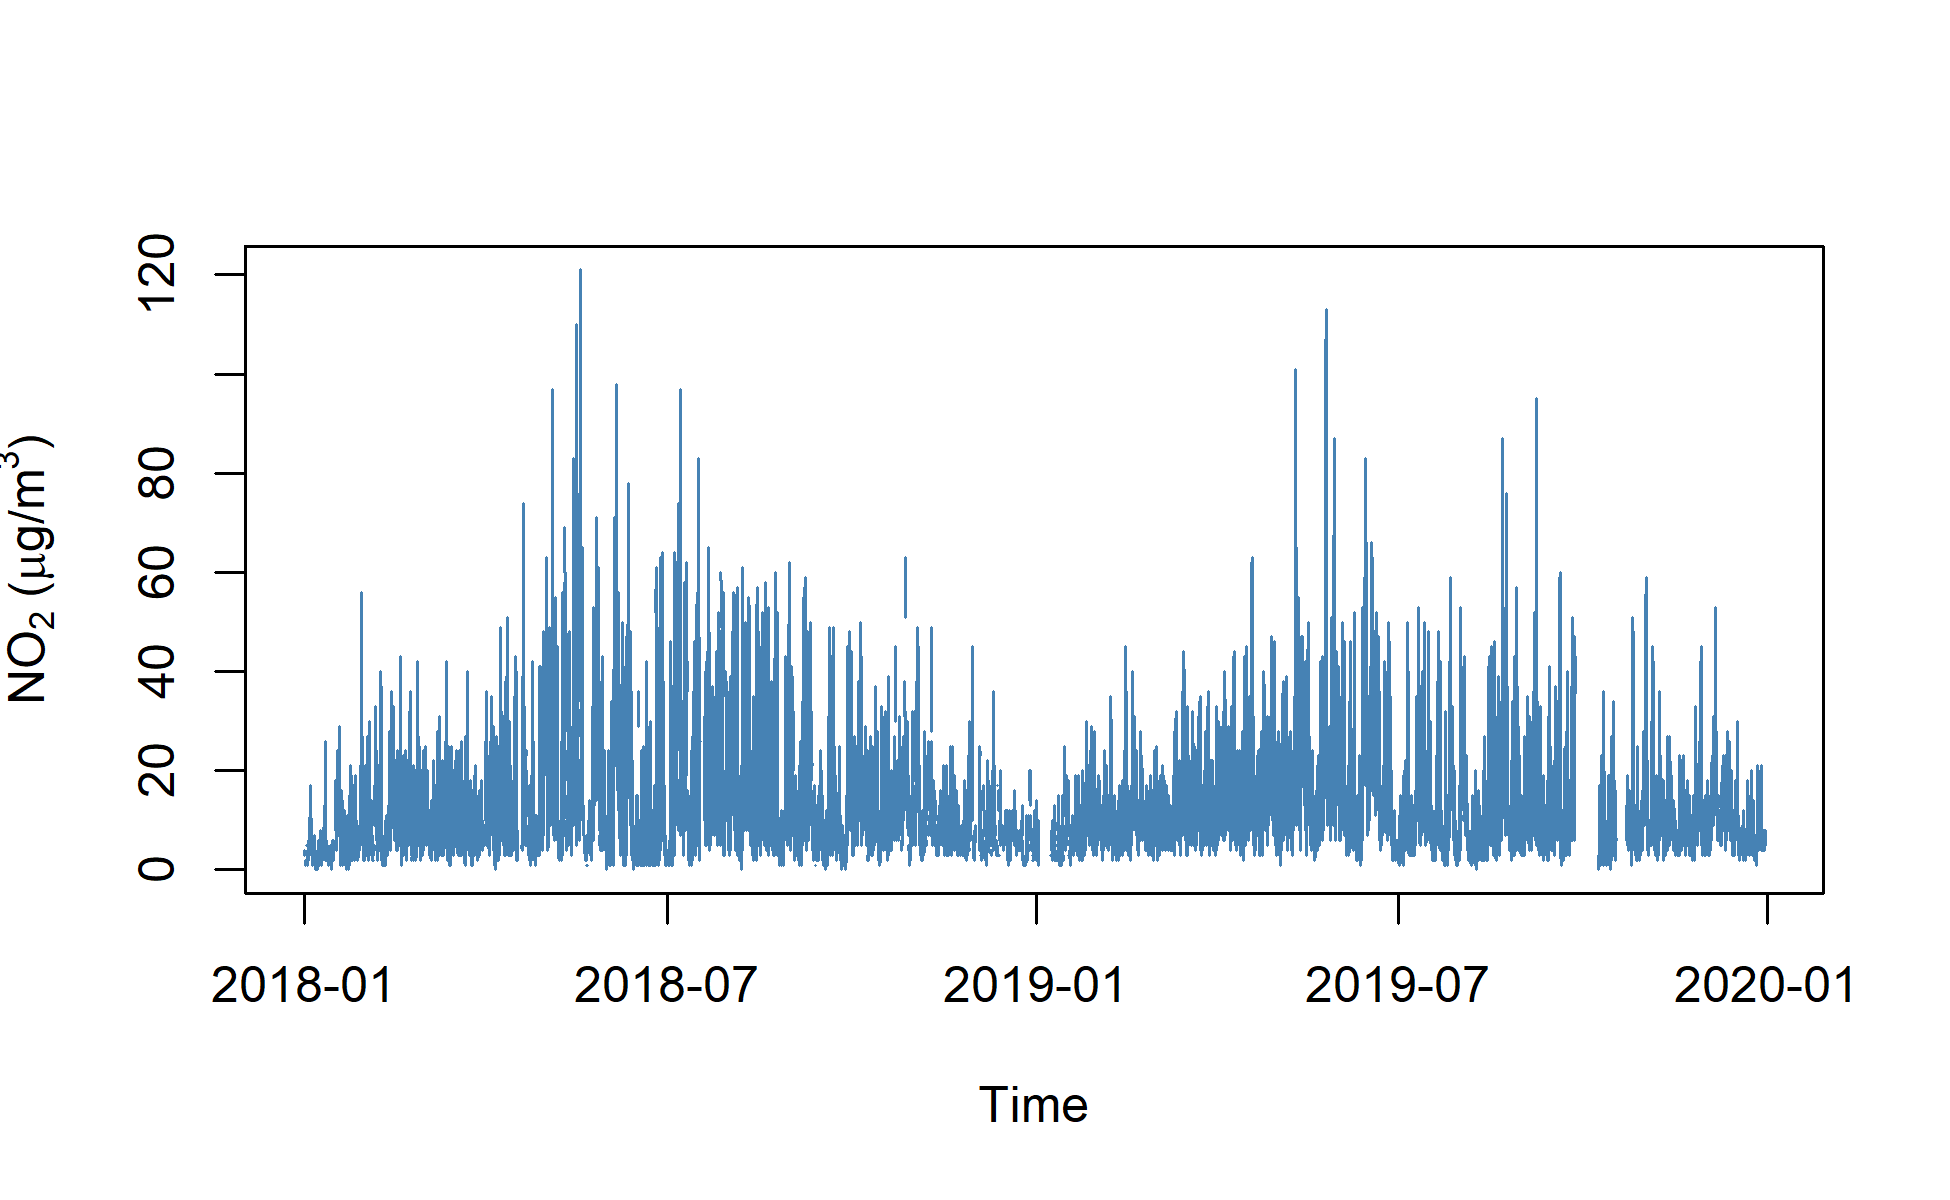
\includegraphics[width=\linewidth]{../img/extracted_no2.png}
            \caption{Before transformations.}
         \end{subfigure}
         \hfill
         \begin{subfigure}{0.48\linewidth}
            \centering
            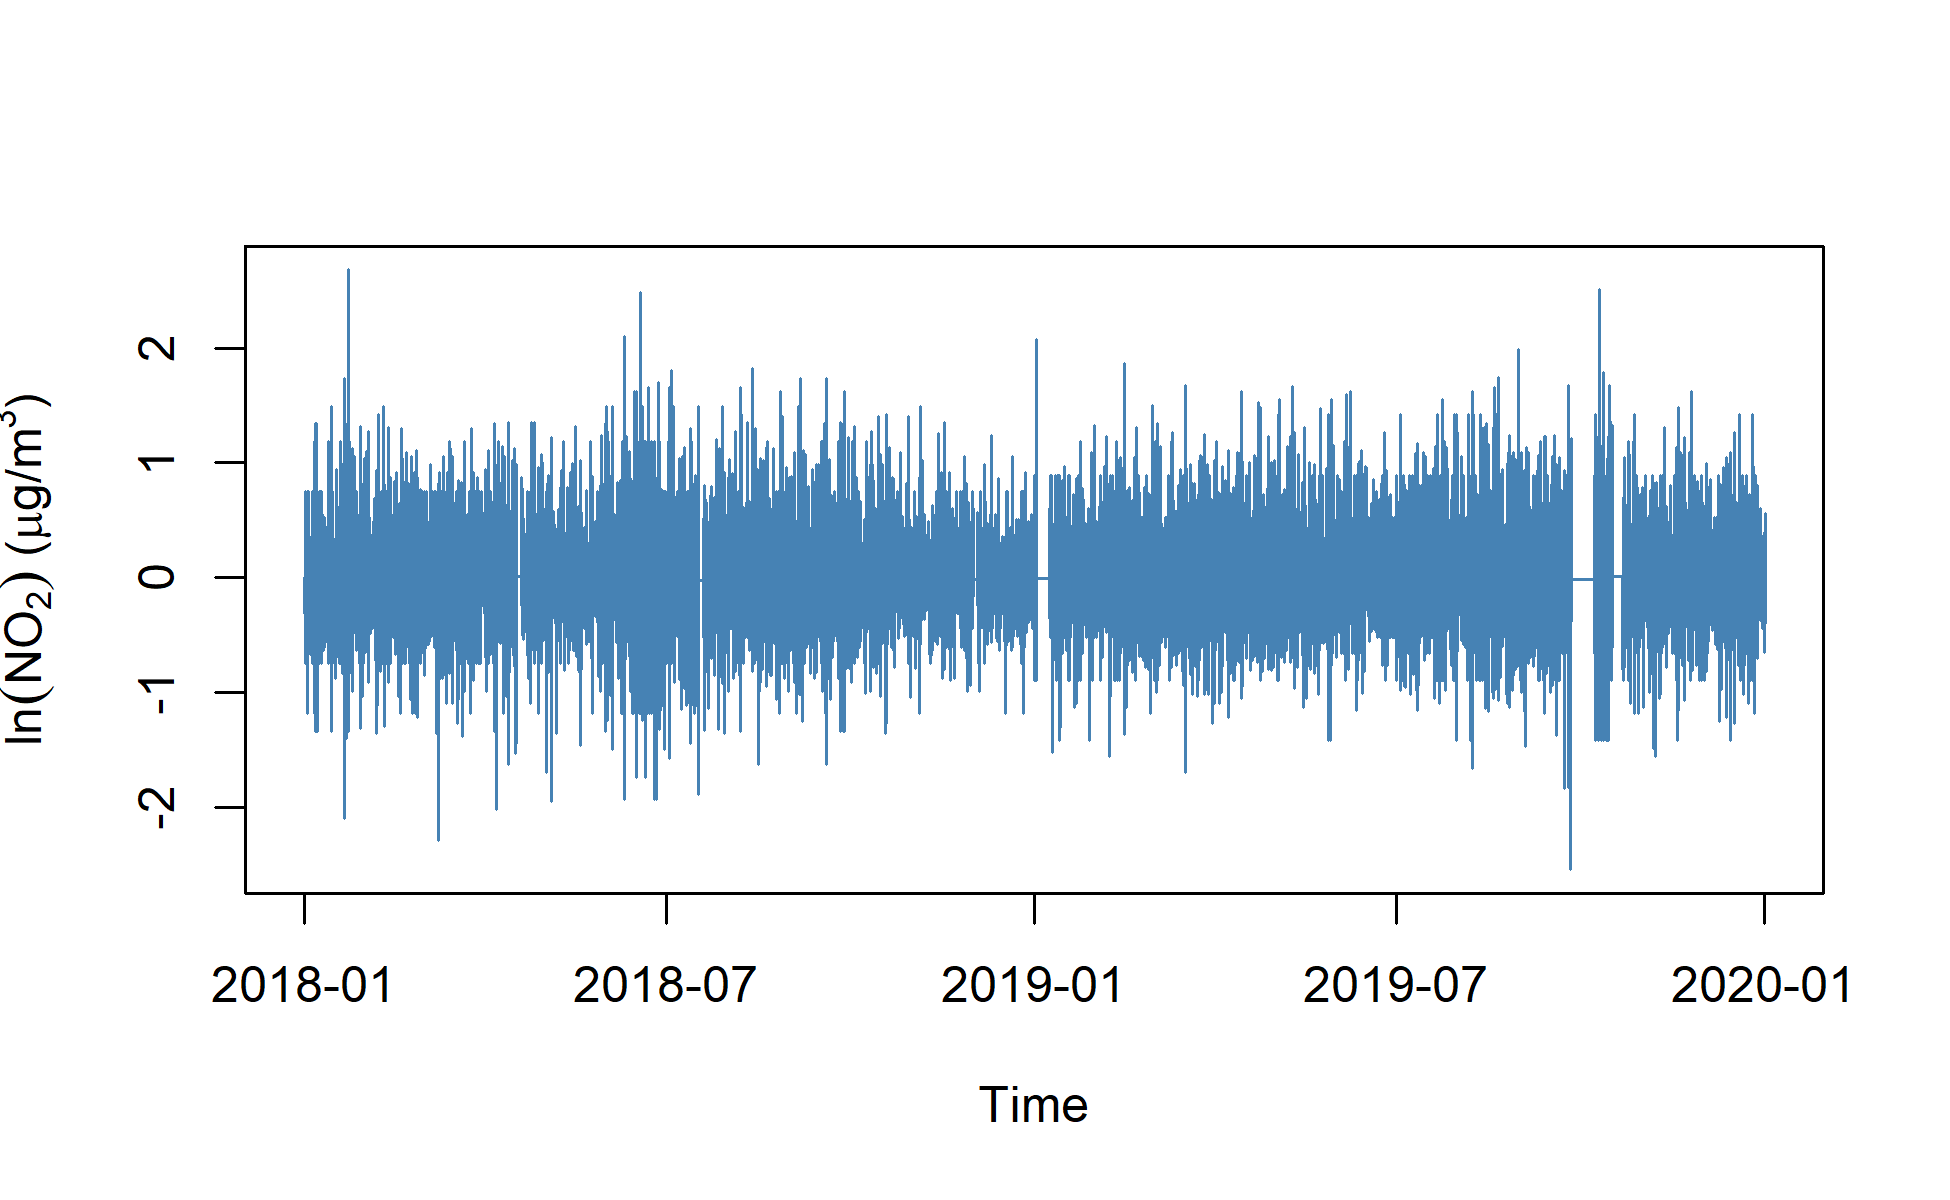
\includegraphics[width=\linewidth]{../img/stationary_no2.png}
            \caption{After transformations.}
         \end{subfigure}
         \caption{\textit{Comparison of NO\textsubscript{2} time series before and after transformations.}}
      \end{figure}

      \subsection*{Model formulation}

         \textbf{Priors}

         \[\alpha \sim \text{half-normal}(0, \, \tau^2)\]
         \begin{align*}
            \pi(\alpha) 
            & = \frac{2}{\sqrt{2\pi\tau^2}} \text{exp}(-\frac{\alpha^2}{2\tau^2})\\
            & \propto \text{exp}(-\frac{\alpha^2}{2\tau^2})\\
            & \text{for } \alpha \geq 0.
         \end{align*}

         \[\rho \sim \text{Inverse-Gamma}(\lambda, \, \beta)\]
         \begin{align*}
            \pi(\rho)
            & = \frac{\beta^{\lambda}}{\Gamma(\lambda)} \rho^{-\lambda-1} \text{exp}(-\frac{\beta}{\rho})\\
            & \propto \rho^{-\lambda-1} \text{exp}(-\frac{\beta}{\rho})\\
            & \text{for } \rho > 0.
         \end{align*}

         \[\sigma \sim \text{half-normal}(0, \, \phi^2)\]
         \begin{align*}
            \pi(\sigma)
            & = \frac{2}{\sqrt{2\pi\phi^2}} \text{exp}(-\frac{\sigma^2}{2\phi^2})\\
            & \propto \text{exp}(-\frac{\sigma^2}{2\phi^2})\\
            & \text{for } \sigma \geq 0.
         \end{align*}

         \textbf{Likelihood}

         \[f(\mathbf{x}) \sim \text{GP}(m(\mathbf{x}) ,\, k(\mathbf{x}, \mathbf{x}'))\]
         \[\mathbf{x} \sim \mathcal{N}_{p}(\mathbf{m} ,\, \mathbf{K})\]
         \begin{align*}
            \mathcal{L}(\mathbf{m} ,\, \mathbf{K} ,\, \mathbf{x}| \, \alpha ,\, \rho ,\, \sigma)
            & = (2\pi)^{-\frac{p}{2}}\text{det}(\mathbf{K})^{-\frac{1}{2}} 
            \text{exp} (-\frac{1}{2} (\mathbf{x} - \mathbf{m})^{\text{\text{T}}} \mathbf{K}^{-1} (\mathbf{x} - \mathbf{m}))\\
            & \propto \text{det}(\mathbf{K})^{-\frac{1}{2}} 
            \text{exp} (-\frac{1}{2} (\mathbf{x} - \mathbf{m})^{\text{\text{T}}} \mathbf{K}^{-1} (\mathbf{x} - \mathbf{m}))\\
            & \text{for } \mathbf{x} \in \mathbb{R}^{p}.
         \end{align*}

         \textbf{Posterior}
         
         \begin{align*}
            \pi(\alpha,\, \rho,\, \sigma| \, \mathbf{x}) 
            & \propto \mathcal{L}(\mathbf{m},\, \mathbf{K},\, \mathbf{x}| \, \alpha,\, \rho,\, \sigma) 
            \cdot \pi(\alpha) 
            \cdot \pi(\rho) 
            \cdot \pi(\sigma)\\
            & \propto \text{det}(\mathbf{K})^{-\frac{1}{2}} 
            \text{exp} (-\frac{1}{2} (\mathbf{x} - \mathbf{m})^{\text{\text{T}}} \mathbf{K}^{-1} (\mathbf{x} - \mathbf{m}))
            \cdot \text{exp}(-\frac{\alpha^2}{2\tau^2}) 
            \cdot \rho^{-\lambda-1} \text{exp}(-\frac{\beta}{\rho}) 
            \cdot \text{exp}(-\frac{\sigma^2}{2\phi^2})\\
            & \text{for } \alpha \geq 0,\ \rho > 0,\ \sigma \geq 0.
         \end{align*}

      \subsection*{Results}

      \begin{table}[H]
         \centering
         \begin{tabular}{lcccccc}
         \hline
         \multirow{2}{*}{Model} & \multicolumn{3}{c}{RMSE} & \multicolumn{3}{c}{MAE} \\
         \cline{2-7}
         & \multicolumn{3}{c}{Forecasts} & \multicolumn{3}{c}{Forecasts} \\
         & \multicolumn{3}{c}{($h$ day time horizon)} & \multicolumn{3}{c}{($h$ day time horizon)} \\
         & 24 & 168 & 744 & 24 & 168 & 744 \\
         \hline
         Average & {7.731} & \textbf{\textcolor{red}{5.397}} & {7.439} & \textbf{\textcolor{red}{6.042}} & \textbf{\textcolor{red}{4.254}} & {5.385} \\
         Naive & {10.553} & {7.864} & {10.040} & {7.708} & {6.071} & {7.308} \\
         Drift & {10.606} & {8.128} & {11.358} & {7.764} & {6.391} & {8.809} \\
         AR(1) & {8.662} & {5.912} & {8.044} & {6.029} & {4.422} & {5.616} \\
         GP-0-WN & {13.756} & {11.141} & {13.169} & {11.719} & {9.786} & {11.081} \\
         GP-0-SE & {~} & {~} & {~} & {~} & {~} & {~} \\
         GP-MLR-WN & \textbf{\textcolor{red}{7.692}} & {6.134} & \textbf{\textcolor{red}{7.225}} & {6.119} & {4.490} & \textbf{\textcolor{red}{5.136}} \\
         GP-MLR-SE & {~} & {~} & {~} & {~} & {~} & {~} \\
         \hline
         \end{tabular}
         \caption{\textit{RMSE and MAE of forecasting models across horizons.}}
      \end{table}

   \section*{Bibliography}
      \begin{enumerate}
         \item \label{Betancourt2020} \href{https://betanalpha.github.io/assets/case_studies/gaussian_processes.html}{Betancourt (2020). Robust Gaussian process modeling.}
          \item \label{Roberts2013} \href{https://royalsocietypublishing.org/}{Roberts et al. (2013). Gaussian processes for time-series modelling. \textit{Philosophical Transactions of the Royal Society}.}
         \item \label{Rasmussen2006} \href{https://gaussianprocess.org/gpml/}{Rasmussen and Williams (2006). Gaussian Processes in Machine Learning. \textit{The MIT Press.}}
      \end{enumerate}
   
   \end{flushleft}
\end{document}
